\documentclass[a4paper,6pt]{article}
\usepackage[utf8]{inputenc}
\usepackage[T1]{fontenc}
\usepackage[left=5mm, right=5mm, top=20mm, bottom=5mm]{geometry}
\usepackage{multicol}
\usepackage{fancyhdr}
\usepackage{sectsty}
\usepackage{amsmath}
\usepackage{setspace}
\usepackage{titlesec}
\usepackage{etoolbox}
\usepackage{mathtools}
\usepackage{multirow}
\usepackage{tikz}
\usepackage{array}

\setlength{\parindent}{0pt}


% Reduziere den Abstand vor und nach align-Umgebungen
\BeforeBeginEnvironment{align}{\vspace{-0.5ex}}
\AfterEndEnvironment{align}{\vspace{-0.5ex}}


% Reduzierung des Zeilenabstandes
\setstretch{0.9}

% Schriftgrösse und Abstand für Überschriften anpassen
\sectionfont{\fontsize{10}{12}\selectfont}
\subsectionfont{\fontsize{8}{10}\selectfont}
\subsubsectionfont{\fontsize{8}{10}\selectfont}
\titlespacing*{\section}{0pt}{1ex plus 1ex minus .2ex}{0.5ex plus .2ex}
\titlespacing*{\subsection}{0pt}{1ex plus 1ex minus .2ex}{0.5ex plus .2ex}
\titlespacing*{\subsubsection}{0pt}{1ex plus 1ex minus .2ex}{0.5ex plus .2ex}

% Kopfzeile
\pagestyle{fancy}
\fancyhf{}
\rhead{Cheat-Sheet GTI}
\lhead{HS23}
\chead{Lukas Batschelet}
\renewcommand{\headrulewidth}{0pt}


\begin{document}
\begin{multicols*}{3}

\section{Notation}
\scriptsize
$$
x \rightarrow y \coloneqq \neg x + y
$$
\begin{center}
\begin{tabular}{c|c|c}
\hline
AND & $\land$ & $\cdot$\\
OR & $\lor$ & $+$ \\
NOT & $\lnot$ & $\overline{x}$ \\
NAND & $\uparrow$ & $\overline{A \cdot B}$ \\
NOR & $\downarrow$ & $\overline{A + B}$ \\
XOR & $\oplus$ & $\neq$ \\
XNOR & $\odot$ & $\equiv$ \\
\hline
\end{tabular}
\end{center}


\section*{Rechengesetze}

\subsection*{Kommutativgesetze}
\begin{align*}
A \cdot B & = B \cdot A \\
A + B & = B + A
\end{align*}

\subsection*{Assoziativgesetze}
\begin{align*}
(A \cdot B) \cdot C & = A \cdot (B \cdot C) \\
(A + B) + C & = A + (B + C)
\end{align*}

\subsection*{Distributivgesetze}
\begin{align*}
A \cdot (B + C) & = (A \cdot B) + (A \cdot C) \\
A + (B \cdot C) & = (A + B) \cdot (A + C)
\end{align*}

\subsection*{Identitätsgesetze}
\begin{align*}
A \cdot 1 & = A \\
A + 0 & = A
\end{align*}

\subsection*{Negationsgesetze}
\begin{align*}
A \cdot \lnot A & = 0 \\
A + \lnot A & = 1
\end{align*}

\subsection*{Idempotenzgesetze}
\begin{align*}
A \cdot A & = A \\
A + A & = A
\end{align*}

\subsection*{Null- und Einselementgesetze}
\begin{align*}
A \cdot 0 & = 0 \\
A + 1 & = 1
\end{align*}

\subsection*{Absorptionsgesetze}
\begin{align*}
A \cdot (A + B) & = A \\
A + (A \cdot B) & = A
\end{align*}

\subsection*{De Morgan'sche Gesetze}
\begin{align*}
\lnot (A \cdot B) & = \lnot A + \lnot B \\
\lnot (A + B) & = \lnot A \cdot \lnot B
\end{align*}

\scriptsize

\section{Beweise}

\subsection*{$\lnot1 = 0$}
\begin{align*}
\lnot1 &= \lnot1 + 0 && \text{(Neutrales Element 0)} \\
   &= \lnot1 + \lnot\lnot0 && \text{(Idempotenz)} \\
   &= \lnot(1 \cdot \lnot0) && \text{(De Morgan)} \\
   &= \lnot\lnot0 && \text{(Neutrales Element 1)} \\
   &= 0 && \text{(Idempotenz)}
\end{align*}

\subsection*{Keine 3-elementige Boolesche Algebra}
Angenommen, es existiert eine 3-elementrige Boolesche Algebra $ M = \{1, 0, a\} $. Für $ \neg a $ gibt es 3 jeweils widersprüchliche Möglichkeiten:
\begin{align*}
\neg a &= 0 & \rightarrow 1 &= a + \neg a = a + 0 = a \\
\neg a &= 1 & \rightarrow 0 &= \neg a \cdot a = 1 \cdot a = a \\
\neg a &= a & \rightarrow 1 &= a + \neg a = a + a = a
\end{align*}

\subsection*{Funktionale Vollständigkeit von $\{\rightarrow, \oplus\}$}
Es ist zu zeigen, dass die Menge $\{\rightarrow, \oplus\}$ funktional vollständig ist, gegeben dass $\{+, \neg\}$ funktional vollständig ist.

Da jede Funktion mit $+$ und $\neg$ darstellbar ist, genügt es zu zeigen, dass sowohl $+$ als auch $\neg$ mit $\rightarrow$ und $\oplus$ ausgedrückt werden können:
\begin{align*}
\neg x &= 1 \oplus x \\
       &= (x \rightarrow x) \oplus x \\
x + y &= \neg x \rightarrow y \\
       &= ((x \rightarrow x) \oplus x) \rightarrow y
\end{align*}

\section*{Digitale Logikbausteine}

\begin{center}
    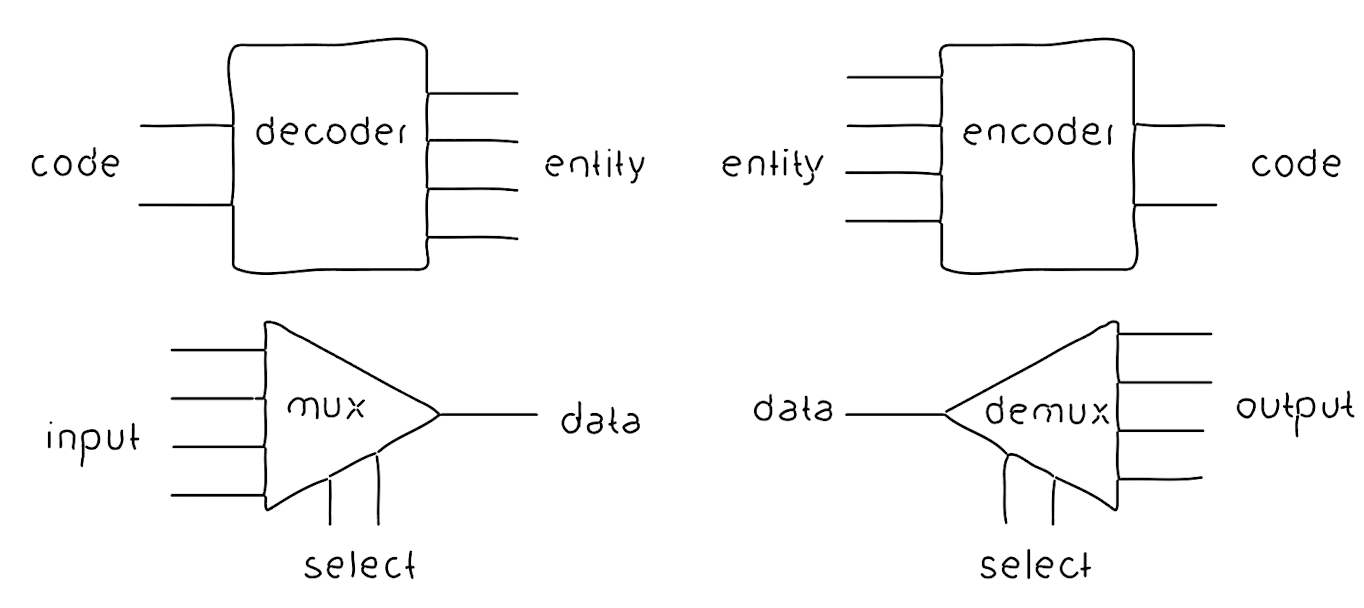
\includegraphics[width=1\linewidth]{resources/Logikbausteine.png}
\end{center}
    

\subsection*{Multiplexer (Mux)}
Ein Multiplexer (Mux) wählt eines von vielen Eingangssignalen aus und leitet dieses auf einen einzelnen Ausgang. Er fungiert als mehrere-zu-eins-Schalter.\\
$ n $ Daten + $ \log_2(n) $ Steuerung
\begin{itemize}
    \item Auswahl eines Datenkanals aus mehreren Quellen.
    \item Routing eines Signals basierend auf einer Steueradresse.
\end{itemize}

\subsection*{Demultiplexer (Demux)}
Ein Demultiplexer (Demux) nimmt ein einzelnes Eingangssignal und leitet es auf eines von vielen Ausgangssignalen. Er funktioniert als eins-zu-mehrere-Schalter.\\
$ \log_2(n) $ Steuerung + $ n $ Ausgänge
\begin{itemize}
    \item Verteilung eines Datenkanals auf mehrere Ausgänge.
    \item Erzeugung mehrerer Steuersignale aus einem einzigen Eingang.
\end{itemize}

\subsection*{Decoder}
Ein Decoder hat $ n $ binäre Eingangsleitungen und $ 2^n $ Ausgangsleitungen. Für jede Eingangskombination wird genau einer der Ausgänge aktiviert. \\
$ n $ Eingänge $ \rightarrow $ $ 2^n $ Ausgänge
\begin{itemize}
    \item Jede Eingangskombination aktiviert genau einen Ausgang.
    \item Einsatz z.B. in digitalen Anzeigesystemen, um eine binäre Zahl in eine spezifische Anzeige zu übersetzen.
\end{itemize}

\subsection*{Encoder}
Ein Encoder hat $ 2^n $ Eingangsleitungen, von denen jeweils nur eine aktiv sein darf, und wandelt diese in eine $ n $-Bit binäre Zahl um. \\
$ 2^n $ Eingänge $ \rightarrow $ $ n $ Ausgänge
\begin{itemize}
    \item Wandelt den aktiven Eingang in eine binäre Darstellung um.
    \item Oft in Tastaturen genutzt, um die gedrückte Taste in einen Binärcode umzuwandeln.
\end{itemize}

\subsection*{Schaltfunktionen}

2-De-Mux (1-to-4-Demultiplexer)
\begin{align*}
    z_0 (x, y_0, y_1) &= x (\neg y_0 \neg y_1) \\
    z_1 (x, y_0, y_1) &= x (\neg y_0 y_1) \\
    z_2 (x, y_0, y_1) &= x ( y_0 \neg y_1) \\
    z_3 (x, y_0, y_1) &= x ( y_0  y_1) 
\end{align*}

\subsection*{Darstellung von Funktionen mittels Multiplexer}

Eine Funktion $ f : B^n \rightarrow B $ kann durch einen $ (n-1) $-Multiplexer dargestellt werden, indem die ersten $ (n-1) $ Variablen als Steuersignale und die $ n $-te Variable als Eingangssignal verwendet werden. Abhängig von den Steuersignalen wird der Mux-Ausgang entweder $ x_n $, $ \neg x_n $, $ 0 $ oder $ 1 $ sein.

Beispiel für $ B^3 \rightarrow B $ mit einem 2-Multiplexer:

\begin{center}
   \begin{tabular}{ccc|c|cc}
    $ x_0 $ & $ x_1 $ & $ x_2 $ & $ z $ & & \\
    \cline{1-6}
    0 & 0 & 0 & 0 & \multirow{2}{*}{$ \rightarrow $} & \multirow{2}{*}{0} \\
    0 & 0 & 1 & 0 & & \\
    \cline{1-6}
    0 & 1 & 0 & 0 & \multirow{2}{*}{$ \rightarrow $} & \multirow{2}{*}{$ x_2 $} \\
    0 & 1 & 1 & 1 & & \\
    \cline{1-6}
    1 & 0 & 0 & 1 & \multirow{2}{*}{$ \rightarrow $} & \multirow{2}{*}{1} \\
    1 & 0 & 1 & 1 & & \\
    \cline{1-6}
    1 & 1 & 0 & 1 & \multirow{2}{*}{$ \rightarrow $} & \multirow{2}{*}{$ \neg x_2 $} \\
    1 & 1 & 1 & 0 & & \\
    \cline{1-6}
    \end{tabular} 
\end{center}


\section*{Basisumwandlung}
$ (132)_{10} \rightarrow (204)_{8}$

\begin{align*}
132 \div 8 &= 16 \text{ Rest } 4 \\
16 \div 8 &= 2 \text{ Rest } 0 \\
2 \div 8 &= 0 \text{ Rest } 2
\end{align*}

\section{Beispielaufgaben}

\subsection{Volladdierer mit 3:8 Decoder}
\tiny
\begin{center}
   \begin{tabular}{ccc|cc}
    \hline
    $A$ & $B$ & $C_{in}$ & $S$ & $C_{out}$ \\ \hline
    0 & 0 & 0   & 0 & 0    \\
    0 & 0 & 1   & 1 & 0    \\
    0 & 1 & 0   & 1 & 0    \\
    0 & 1 & 1   & 0 & 1    \\
    1 & 0 & 0   & 1 & 0    \\
    1 & 0 & 1   & 0 & 1    \\
    1 & 1 & 0   & 0 & 1    \\
    1 & 1 & 1   & 1 & 1    \\ \hline
    \end{tabular} 
\end{center}

\scriptsize

\begin{center}
    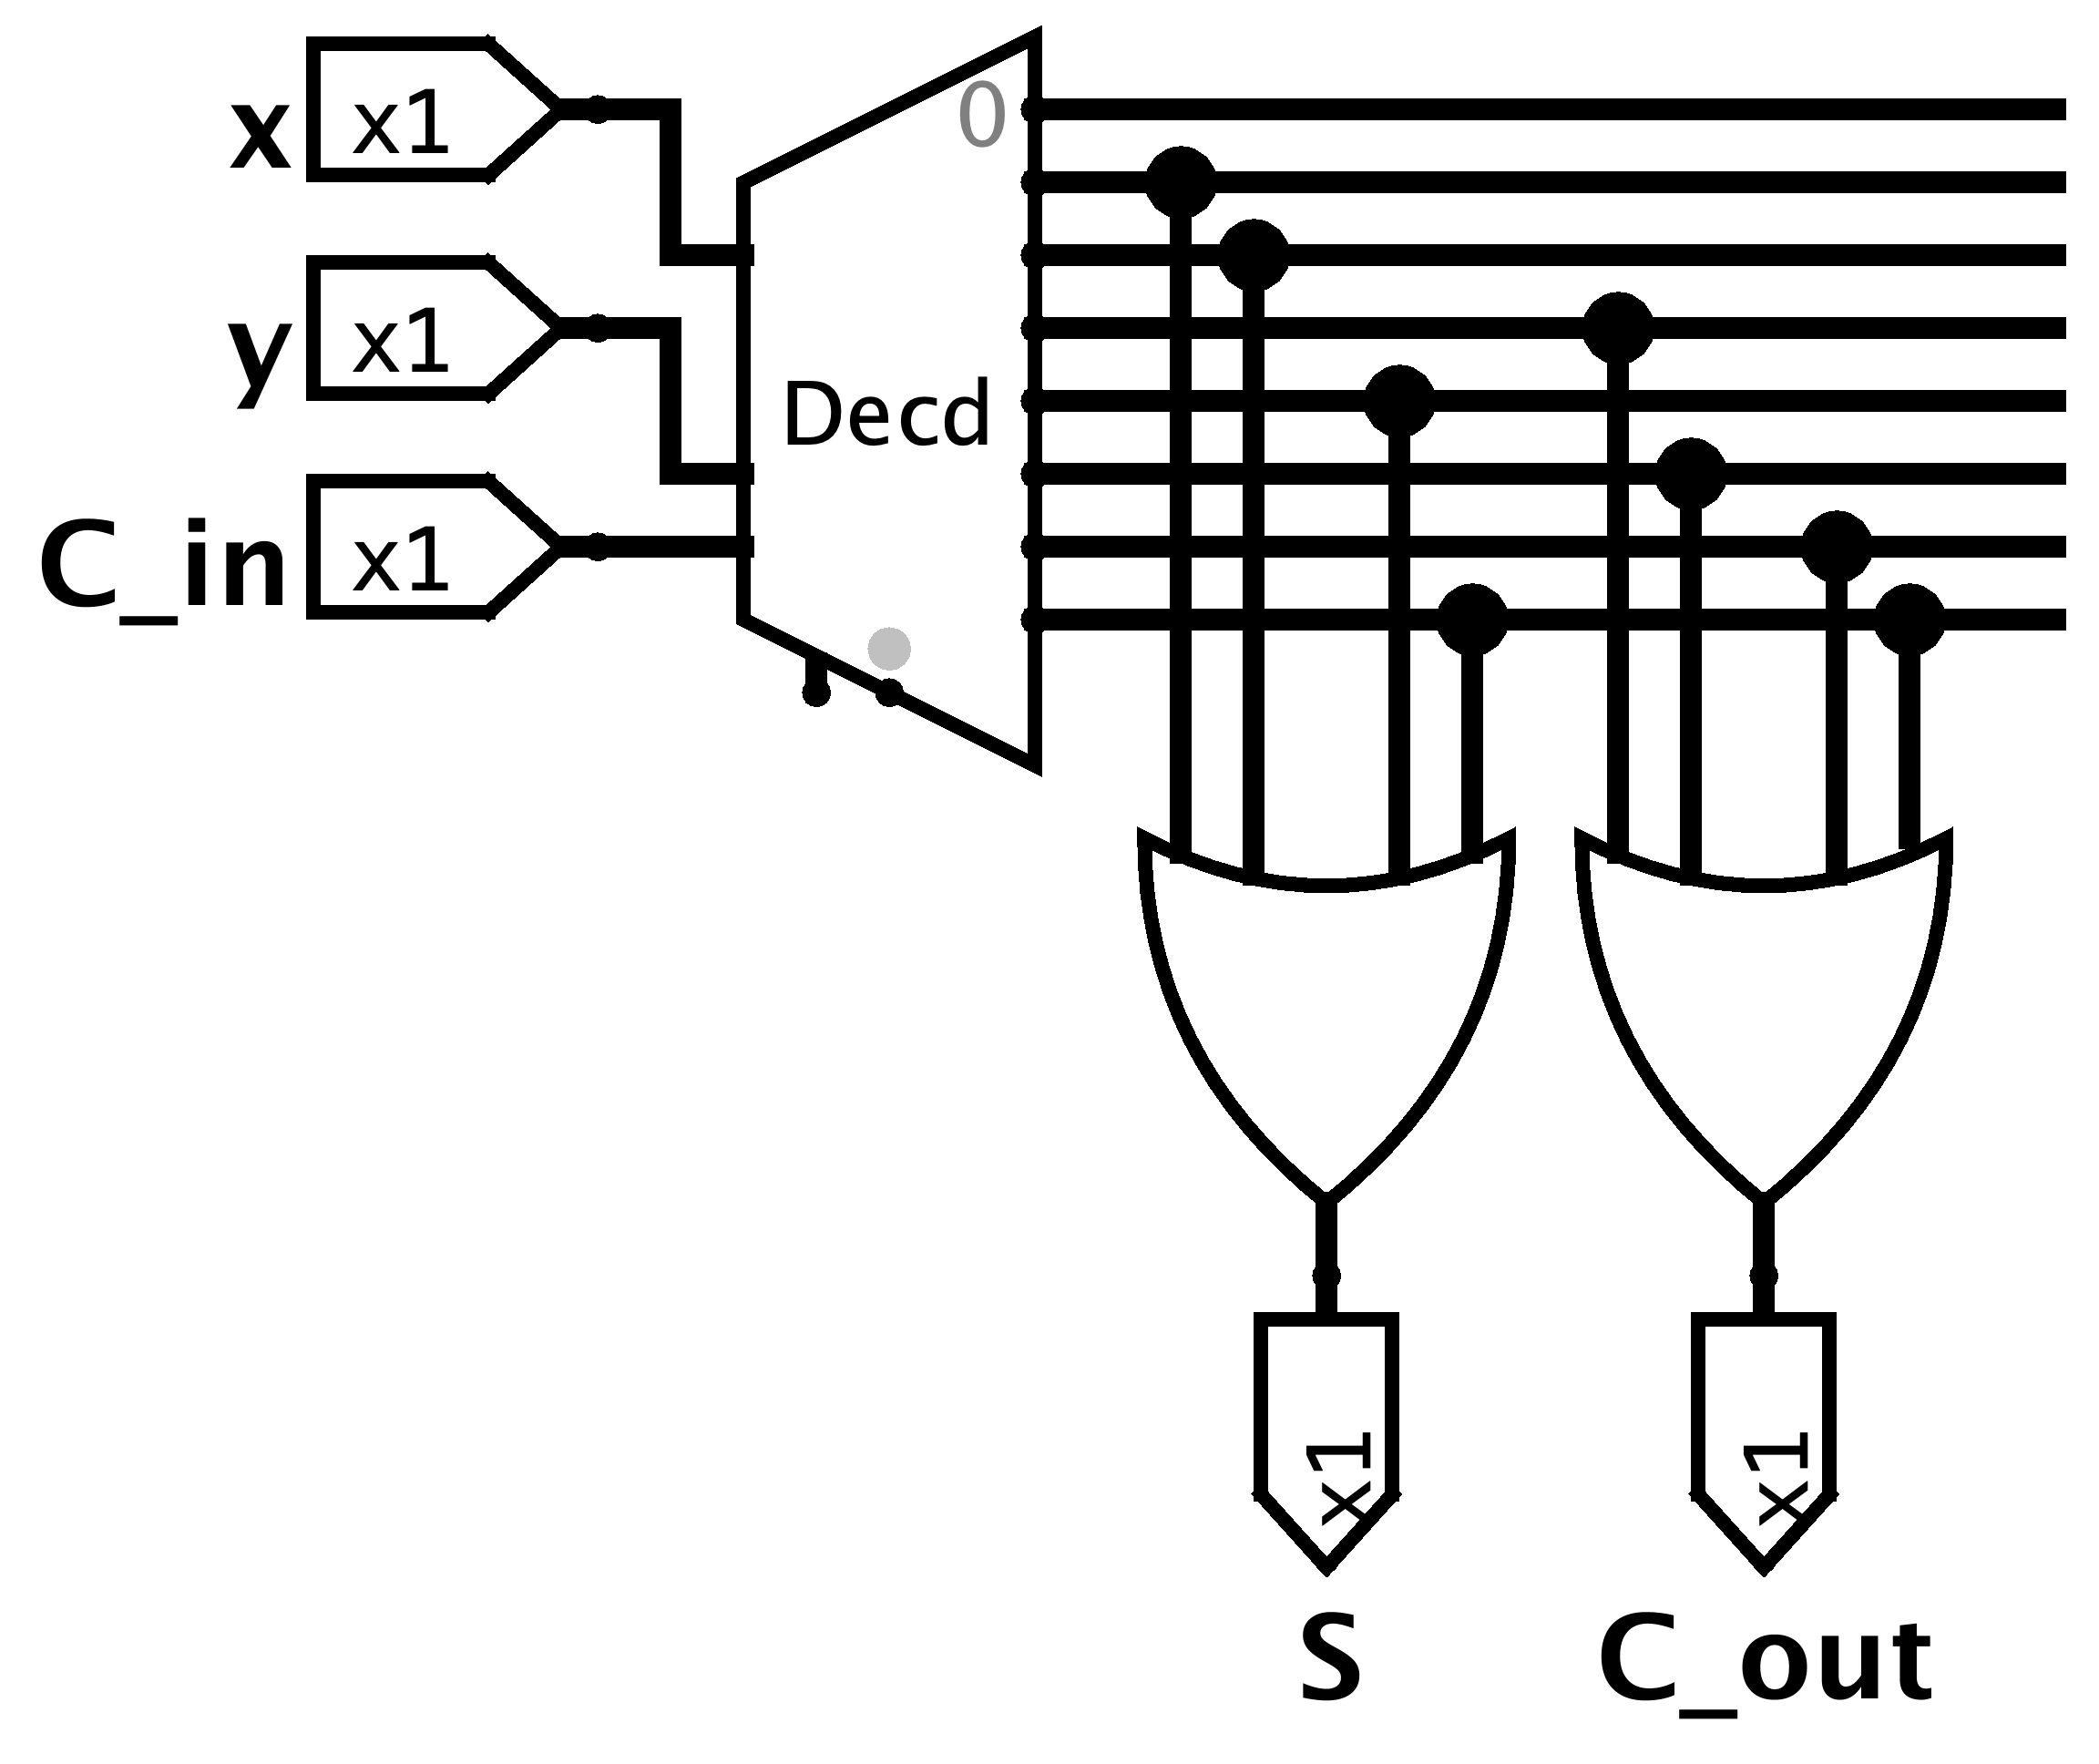
\includegraphics[width=0.75\linewidth]{resources/Decoder_Full_Adder.png}
\end{center}
    

\subsection{Quine McCluskey Verfahren}
\small
$$
f(a,b,c,d) = \sum m(0,1,2,5,6,7,8,9,10,14)
$$
\scriptsize

\begin{center}
    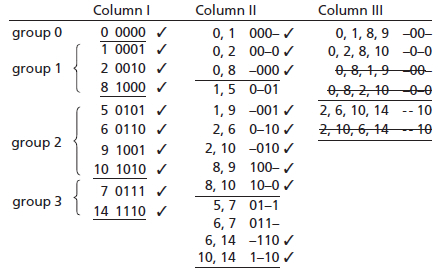
\includegraphics[width=1\linewidth]{resources/prime_implicants_table Kopie.jpg}
\end{center}

Nicht weiter verwendete Minterme:
$$ f = \overline{a} \overline{c} d + \overline{a} b \overline{d} + \overline{a} b c + \overline{b} \overline{c} + \overline{b} \overline{d} + c \overline{d}$$

\scriptsize

% Definiere einen neuen Spaltentyp 'C', der eine zentrierte Spalte einer bestimmten Breite erstellt
\newcolumntype{C}[1]{>{\centering\arraybackslash}p{#1}}

% Hier würde man die Breite anpassen, um die optimale Passform zu finden
\newcommand\mintermwidth{0.07cm}

\begin{tabular}{c|*{10}{C{\mintermwidth}|}}
    \textbf{Term}                     & 0 & 1 & 2 & 5 & 6 & 7 & 8 & 9 & 10& 14 \\ \hline
    $\overline{a} \overline{c} d$     &   & 1 &   & 1 &   &   &   &   &   &   \\ \hline
    $\overline{a} b d$                &   &   &   & \textbf{1} &   & \textbf{1} &   &   &   &   \\ \hline
    $\overline{a} b c$                &   &   &   &   & 1 & 1 &   &   &   &   \\ \hline
    $\overline{b} \overline{c}$       & \textbf{1} & \textbf{1} &   &   &   &   & \textbf{1} & \textbf{1} &   &   \\ \hline
    $\overline{b} \overline{d}$       & 1 &   & 1 &   &   &   & 1 &   & 1 &   \\ \hline
    $c \overline{d}$                  &   &   & \textbf{1} &   & \textbf{1} &   &   & \textbf{1} & \textbf{1} & \textbf{1} \\ \hline
\end{tabular}

\scriptsize

Minimale Darstellung:
$$f = \overline{a}bd + \overline{b}\overline{c} + c\overline{d}$$


\subsection{OBDD}

\scriptsize
\begin{tabular}{ccc|c}
    \hline
    x & y & z & $f(x,y,z)$ \\
    \hline
    0 & 0 & 0 & 1 \\
    0 & 0 & 1 & 0 \\
    0 & 1 & 0 & 0 \\
    0 & 1 & 1 & 0 \\
    1 & 0 & 0 & 0 \\
    1 & 0 & 1 & 0 \\
    1 & 1 & 0 & 1 \\
    1 & 1 & 1 & 0 \\
    \hline
\end{tabular}

\scriptsize

OBDD mit $x > z > y$

\begin{center}
    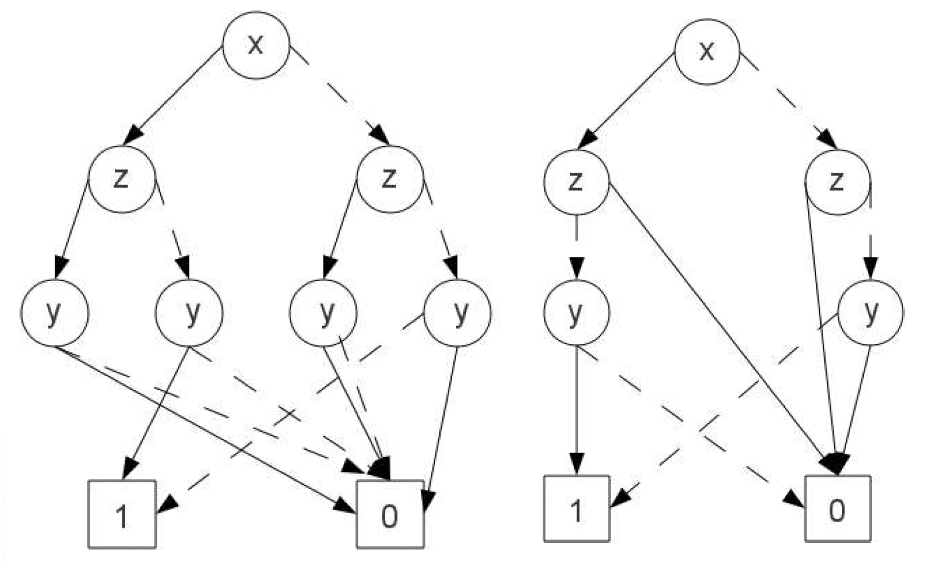
\includegraphics[width=1\linewidth]{resources/OBDD.png}
\end{center}

Optimiertes OBDD mit $z > y > x$

\begin{center}
    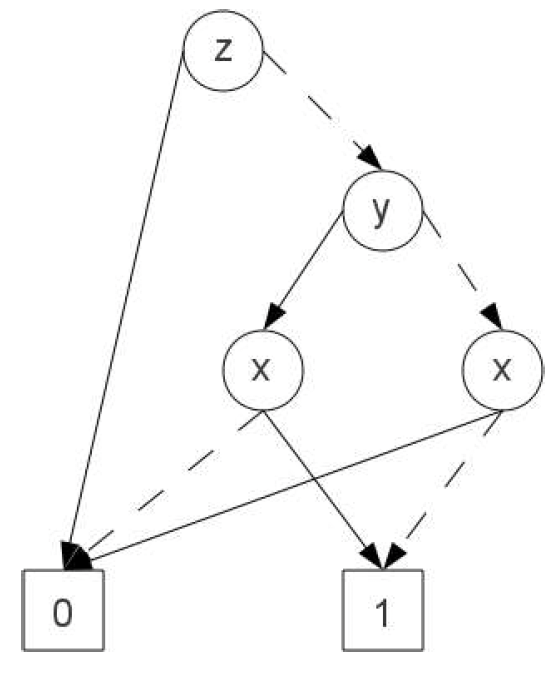
\includegraphics[width=0.5\linewidth]{resources/Optimiertes_OBDD.png}
\end{center}

\scriptsize


\subsection{Unabhängige Fehlerdiagnose}
\[ f(x_0, x_1, x_2) = x_0(x_1 + \overline{x_2}) \]

\scriptsize
Wertetabelle:

\tiny
\begin{center}
    \begin{tabular}{ccc|c}
        \hline
        $x_0$ & $x_1$ & $x_2$ & $f(x_0, x_1, x_2)$ \\
        \hline
        0 & 0 & 0 & 0 \\
        0 & 0 & 1 & 0 \\
        0 & 1 & 0 & 0 \\
        0 & 1 & 1 & 0 \\
        1 & 0 & 0 & 1 \\
        1 & 0 & 1 & 0 \\
        1 & 1 & 0 & 1 \\
        1 & 1 & 1 & 1 \\
        \hline
    \end{tabular}
\end{center}


\scriptsize

Testpaare:

\begin{itemize}
    \item $x_0$: \{(000), (100)\}, \{(010), (110)\}, \{(011), (111)\}
    \item $x_1$: \{(101), (111)\}
    \item $x_2$: \{(100), (101)\}
\end{itemize}

Minimale Testmengen:

\begin{itemize}
    \item \{(000), (100), (101), (111)\}
    \item \{(011), (100), (101), (111)\}
\end{itemize}

\subsection{Eliminieren von Schaltungshazards}

Anwenden von Satz von Eichelberger. Alle Primimplikanten in DNF führt zu Hazard-freiem Verhalten.

\subsection{Schaltungsabhängige Fehlerdiagnose}

$$
f(x_0, x_1) = x_0 \oplus x_1
$$

Annahme: \quad $f_{x_0} = x_0$ Stuck \@ zero

\qquad \qquad \qquad $f_{x_1} = x_1$ Stuck \@ zero 

\tiny
    \begin{center}
        \begin{tabular}{cc|c|cc}
            \hline
            $x_0$ & $x_1$ & $f$ & $f_{x_0}$ & $f_{x_1}$\\
            \hline
            0 & 0 & 0 & 0 & 0 \\
            0 & 1 & 1 & 1 & 0 \\
            1 & 0 & 1 & 0 & 1 \\
            1 & 1 & 0 & 1 & 1 \\
            \hline
        \end{tabular}
    \end{center}    
\scriptsize

\tiny
    \begin{center}
        \begin{tabular}{cc|c|cc}
            \hline
            $x_0$ & $x_1$ & $f$ & $f \oplus f_{x_0}$ & $f \oplus f_{x_1}$\\
            \hline
            0 & 0 & 0 & 0 & 0 \\
            0 & 1 & 1 & 0 & \textbf{1} \\
            1 & 0 & 1 & \textbf{1} & 0 \\
            1 & 1 & 0 & \textbf{1} & \textbf{1} \\
            \hline
        \end{tabular}
    \end{center}    
\scriptsize

Minimale Testmenge:

\begin{itemize}
    \item $\{(1,1)\}$
\end{itemize}
Alle Fehler sind feststellbar.

\section{Delays}

\begin{center}
    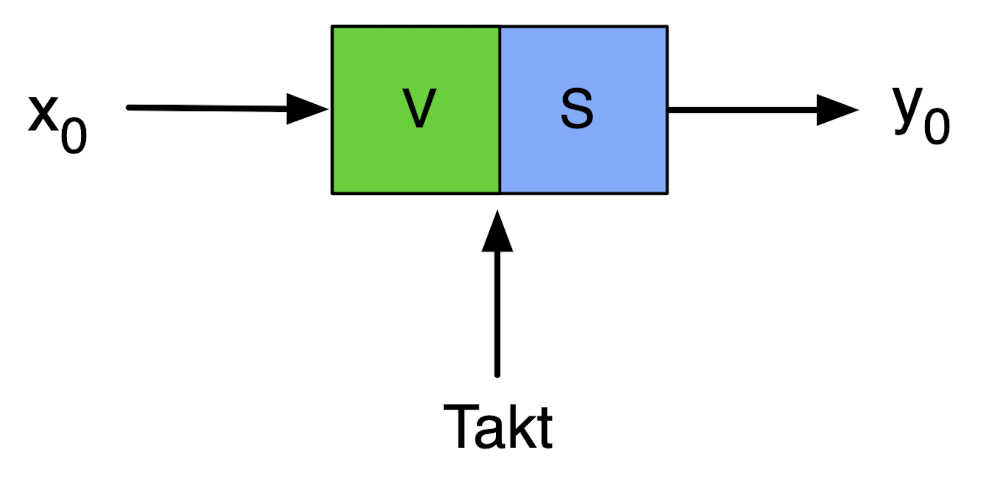
\includegraphics[width=0.5\linewidth]{resources/Bildschirmfoto 2024-01-04 um 10.25.00.png}
\end{center}

\begin{itemize}
    \item Synchronisiertes Delay durch zentrale Uhr
    \item Taktimpulse steuern Rückkopplungs-Delay
    \item Sperrschaltung zwischen Vor- und Hauptspeicher
    \item Arbeitsphase: Ausgabe des Hauptspeichers (S)
    \item Setzphase: Übertrag von Vor- (V) zu Hauptspeicher (S)
    \item Kurzzeitiges Öffnen der Sperre während Setzphase
\end{itemize}

\subsection{Flipflops}

\subsubsection{SR-Flipflop}

\begin{center}
    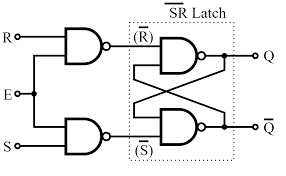
\includegraphics[width=0.75\linewidth]{resources/SR_FlipFlop_CLK.png}
\end{center}

\begin{itemize}
    \item Zwei Eingänge: Set (S), Reset (R)
    \item Flanken- oder pegelgesteuert konfigurierbar
    \item Flankensteuerung: Zusätzliche Logik (z.B. Taktflankendetektor)
    \item Vermeiden von gleichzeitigem S=R=1
    \item Race Condition, falls $S$ und $R$ fast gleichzeitig von 0 auf 1 wechseln
    \item Master-Slave für definierte Ausgabe bei Flanke
    \item[$\rightarrow$] Anlegen eines \textbf{Taktsignals} erlaubt bessere Kontrolle.
\end{itemize}

\begin{center}
    \begin{tabular}{|c|c||c|c|}
    \hline
    $S$ & $R$ & $Q(t_0)$ & $Q(t_1)$ \\ \hline
    0 & 0 & 0 & 0 \\ \hline
    0 & 0 & 1 & 1 \\ \hline
    0 & \textbf{1} & 0 & \textbf{0} \\ \hline
    0 & \textbf{1} & 1 & \textbf{0} \\ \hline
    \textbf{1} & 0 & 0 & \textbf{1} \\ \hline
    \textbf{1} & 0 & 1 & \textbf{1} \\ \hline
    \textbf{1} & \textbf{1} & \multicolumn{2}{c|}{\textbf{verboten}} \\ \hline
    \end{tabular}
\end{center}

\subsubsection{D-Flipflop}




\begin{center}
    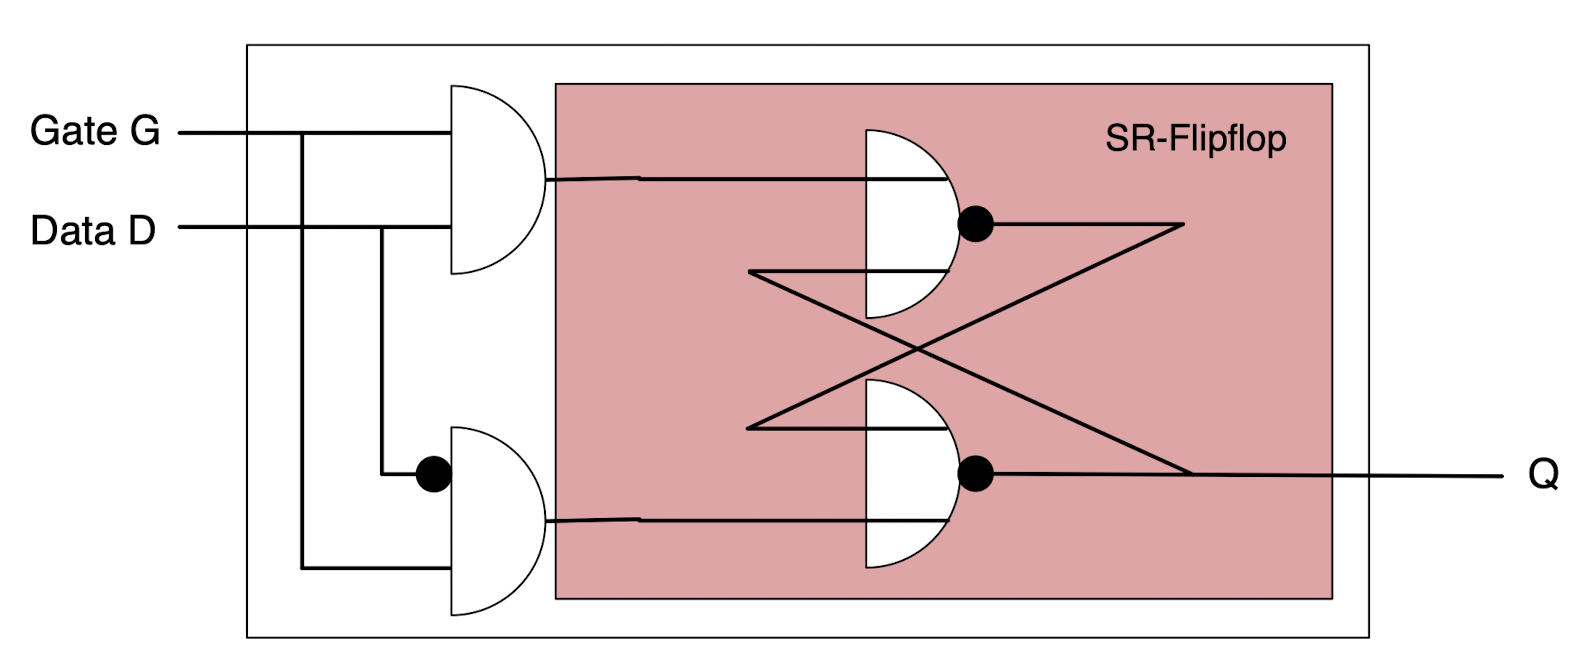
\includegraphics[width=1\linewidth]{resources/Bildschirmfoto 2024-01-03 um 16.50.26.png}
    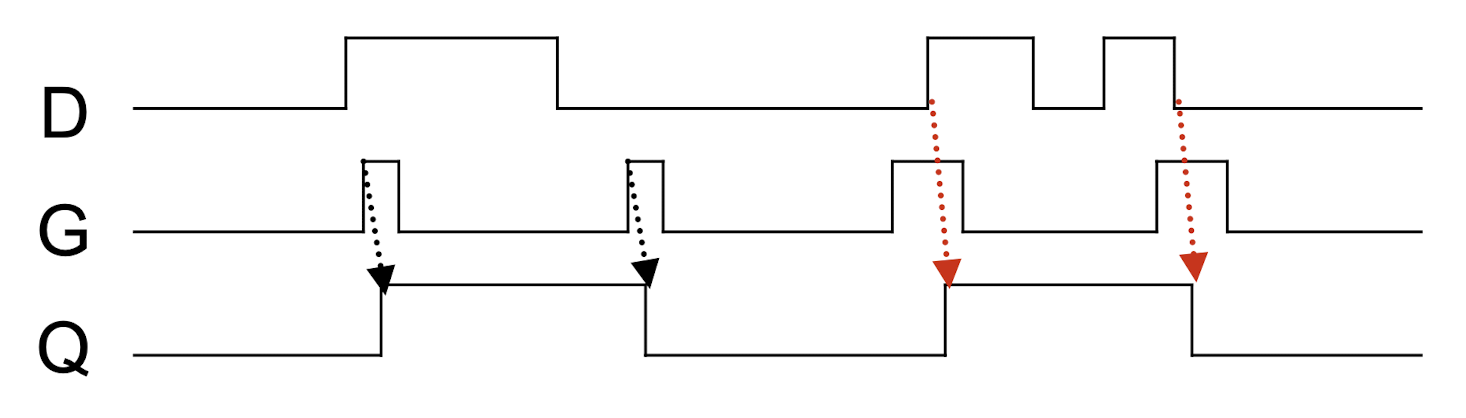
\includegraphics[width=1\linewidth]{resources/Bildschirmfoto 2024-01-03 um 16.51.26.png}
\end{center}

\begin{itemize}
    \item Ein Daten-Eingang (D), ein Takt-Eingang (Clock)
    \item Flankengetriggert: Übernahme von D bei Taktflanke
    \item Keine verbotenen Zustände
    \item Speichert einzelnes Bit
    \item Auch in Master Slave Schaltung möglich (Edge-Triggered)
\end{itemize}

\begin{center}
    \begin{tabular}{|c|c||c|c|}
    \hline
    $D$ & $G$ & $Q(t_0)$ & $Q(t_1)$ \\ \hline
    0 & 0 & 0 & 0 \\ \hline
    0 & 0 & 1 & 1 \\ \hline
    0 & \textbf{1} & 0 & \textbf{0} \\ \hline
    0 & \textbf{1} & 1 & \textbf{0} \\ \hline
    1 & 0 & 0 & 0 \\ \hline
    1 & 0 & 1 & 1 \\ \hline
    \textbf{1} & \textbf{1} & 0 & \textbf{1} \\ 
    \textbf{1} & \textbf{1} & 1 & \textbf{1} \\ \hline
    \end{tabular}
\end{center}

\subsubsection{JK-Fliflop}



\begin{center}
    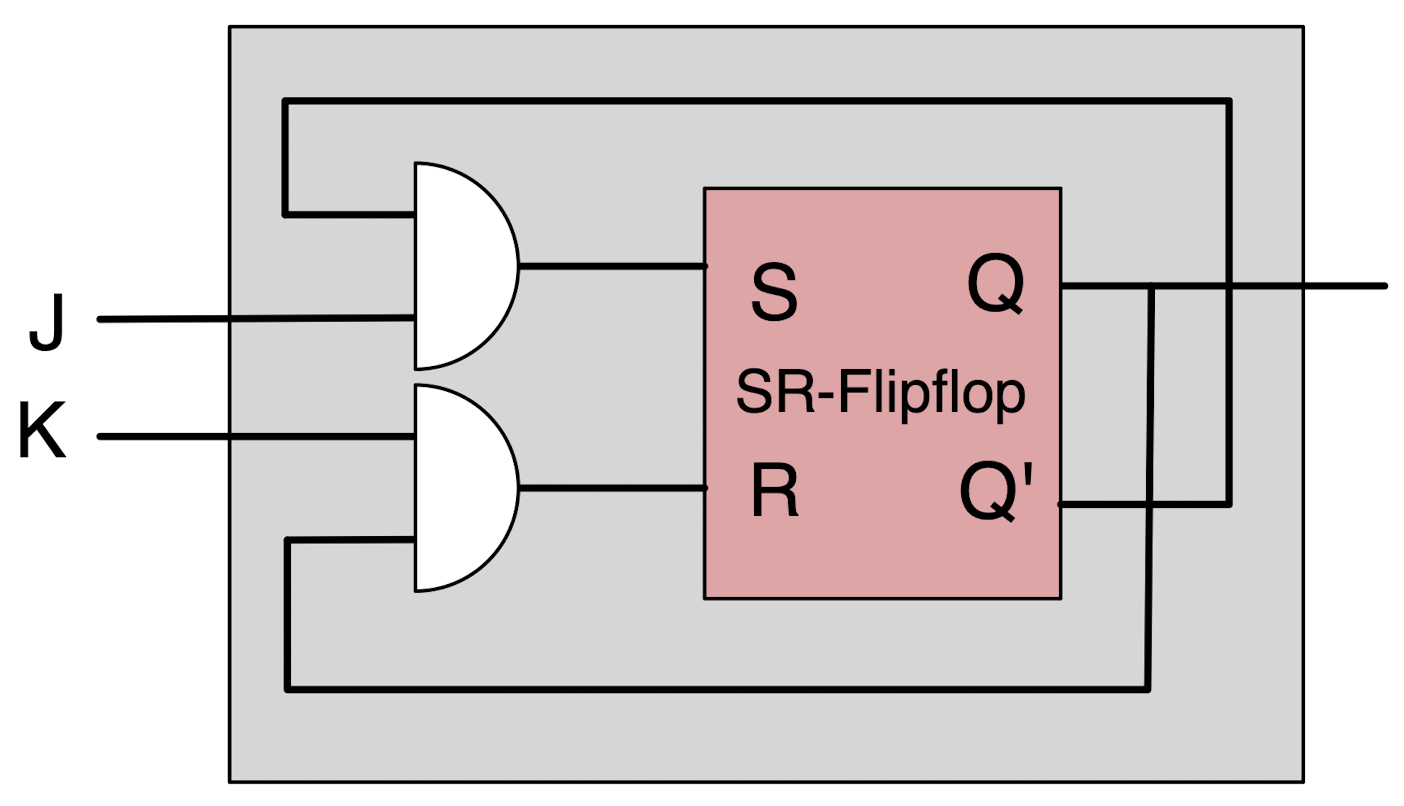
\includegraphics[width=0.75\linewidth]{resources/Bildschirmfoto 2024-01-04 um 08.26.25.png}
\end{center}

\begin{itemize}
    \item Zwei Eingänge: J (Set), K (Reset)
    \item Flankengetriggert: Toggeln bei J=K=1
    \item Interne Rückkopplung verhindert undefinierte Zustände
    \item Master-Slave-Variante für sequenzielle Logik
    \item Geeignet für Zähler und Register
    \item Setzen nur möglich wenn $Q = 0$, Reset nur möglich wenn $Q = 1$
\end{itemize}

\begin{center}
    \begin{tabular}{|c|c|c|c||c|c|}
    \hline
    J & K & S & R & $Q(t_0)$ & $Q(t_1)$ \\ \hline
    0 & 0 & 0 & 0 & 0 & 0 \\ \hline
    0 & 0 & 0 & 0 & 1 & 1 \\ \hline
    0 & 1 & 0 & 0 & 0 & 0 \\ \hline
    0 & 1 & 0 & 1 & 1 & 0 \\ \hline
    1 & 0 & 1 & 0 & 0 & 1 \\ \hline
    1 & 0 & 0 & 0 & 1 & 1 \\ \hline
    1 & 1 & 1 & 0 & 0 & 1 \\ \hline
    1 & 1 & 0 & 1 & 1 & 0 \\ \hline
    \end{tabular}
\end{center}

\subsection{MUX-Delay}

\begin{center}
    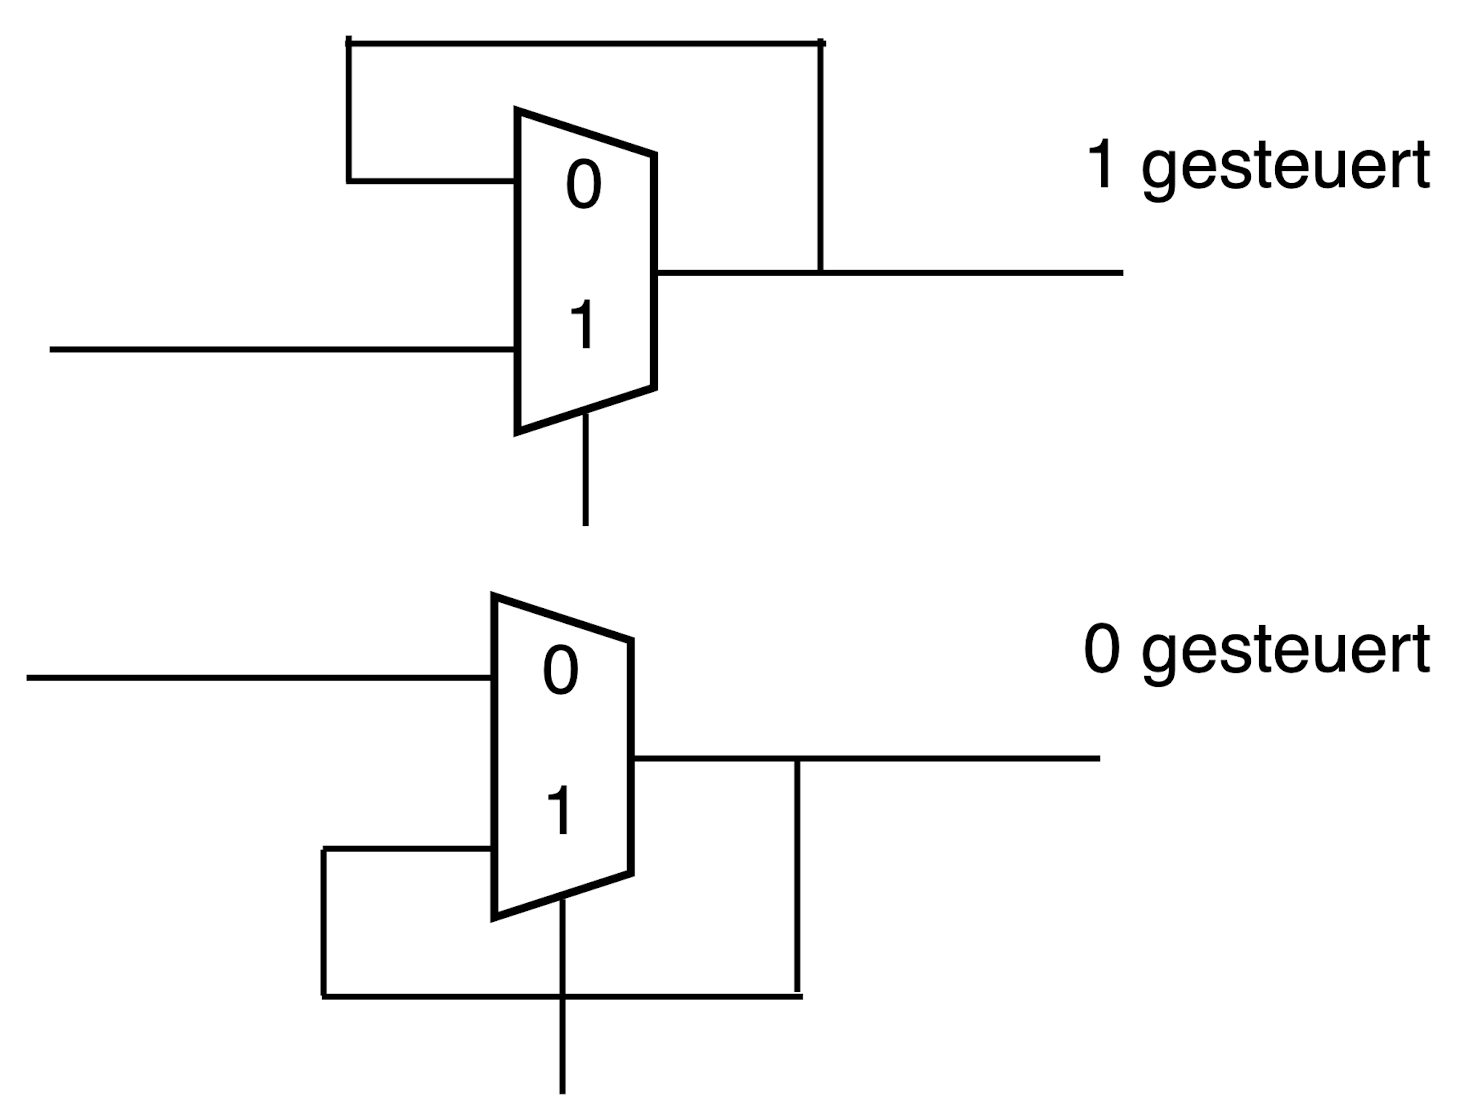
\includegraphics[width=0.75\linewidth]{resources/Bildschirmfoto 2024-01-04 um 10.36.08.png}
\end{center}

\begin{itemize}
    \item MUX Delay: Zeitverzögerung beim Durchschalten der Daten.
    \item MUX Konfiguration für einfache Flanke: Takt direkt an Steuereingang.
    \item MUX Konfiguration für doppelte Flanke: Takt und invertierter Takt auf Steuereingänge zweier MUXe, die abwechselnd aktiviert werden.
\end{itemize}

\section{Schaltwerke}

\subsection*{Einer- und Zweierkomplement}

\textbf{Einerkomplement:}
\begin{itemize}
    \item Invertierung jedes Bits (0 wird zu 1, 1 wird zu 0).
    \item Beispiel: Einerkomplement von 0101 ist 1010.
    \item Zwei Darstellungen für Null (0000 und 1111).
    \item "Overflow" wird an der niedrigsten Stelle addiert.
\end{itemize}

\begin{align*}
    & \textit{Beispiel:} \quad -63_{(10)} - 27_{(10)} \\
    & -63_{(10)} \rightarrow  -(0011\ 1111)_{(2)} \rightarrow 1100\ 0000_{(2)} \\
    & -27_{(10)} \rightarrow  -(0001\ 1011)_{(2)} \rightarrow 1110\ 0100_{(2)} \\
    & \begin{array}{r@{}c@{}l}
        &1100\ 0000_{(2)} & \\
        +&1110\ 0100_{(2)} & \\
        \cline{1-2}
        1&1010\ 0100_{(2)} & \rightarrow 1010\ 0101_{(2)} \\
        \cline{1-2}
        \\
        &1010\ 0101_{(2)} & \rightarrow -(0101\ 1010)_{(2)} \rightarrow -90_{(10)}
    \end{array}
\end{align*}

\textbf{Zweierkomplement:}
\begin{itemize}
    \item Addition von 1 zum Einerkomplement.
    \item Beispiel: Zweierkomplement von 0101 ist 1011.
    \item Eine Darstellung für Null, vereinfacht binäre Subtraktion.
    \item[!] Aufpassen beim zurückwandeln, auch hier wieder $+1$ 
\end{itemize}


\subsection*{3-Bit Addier-/Subtrahierwerk}

\begin{center}
    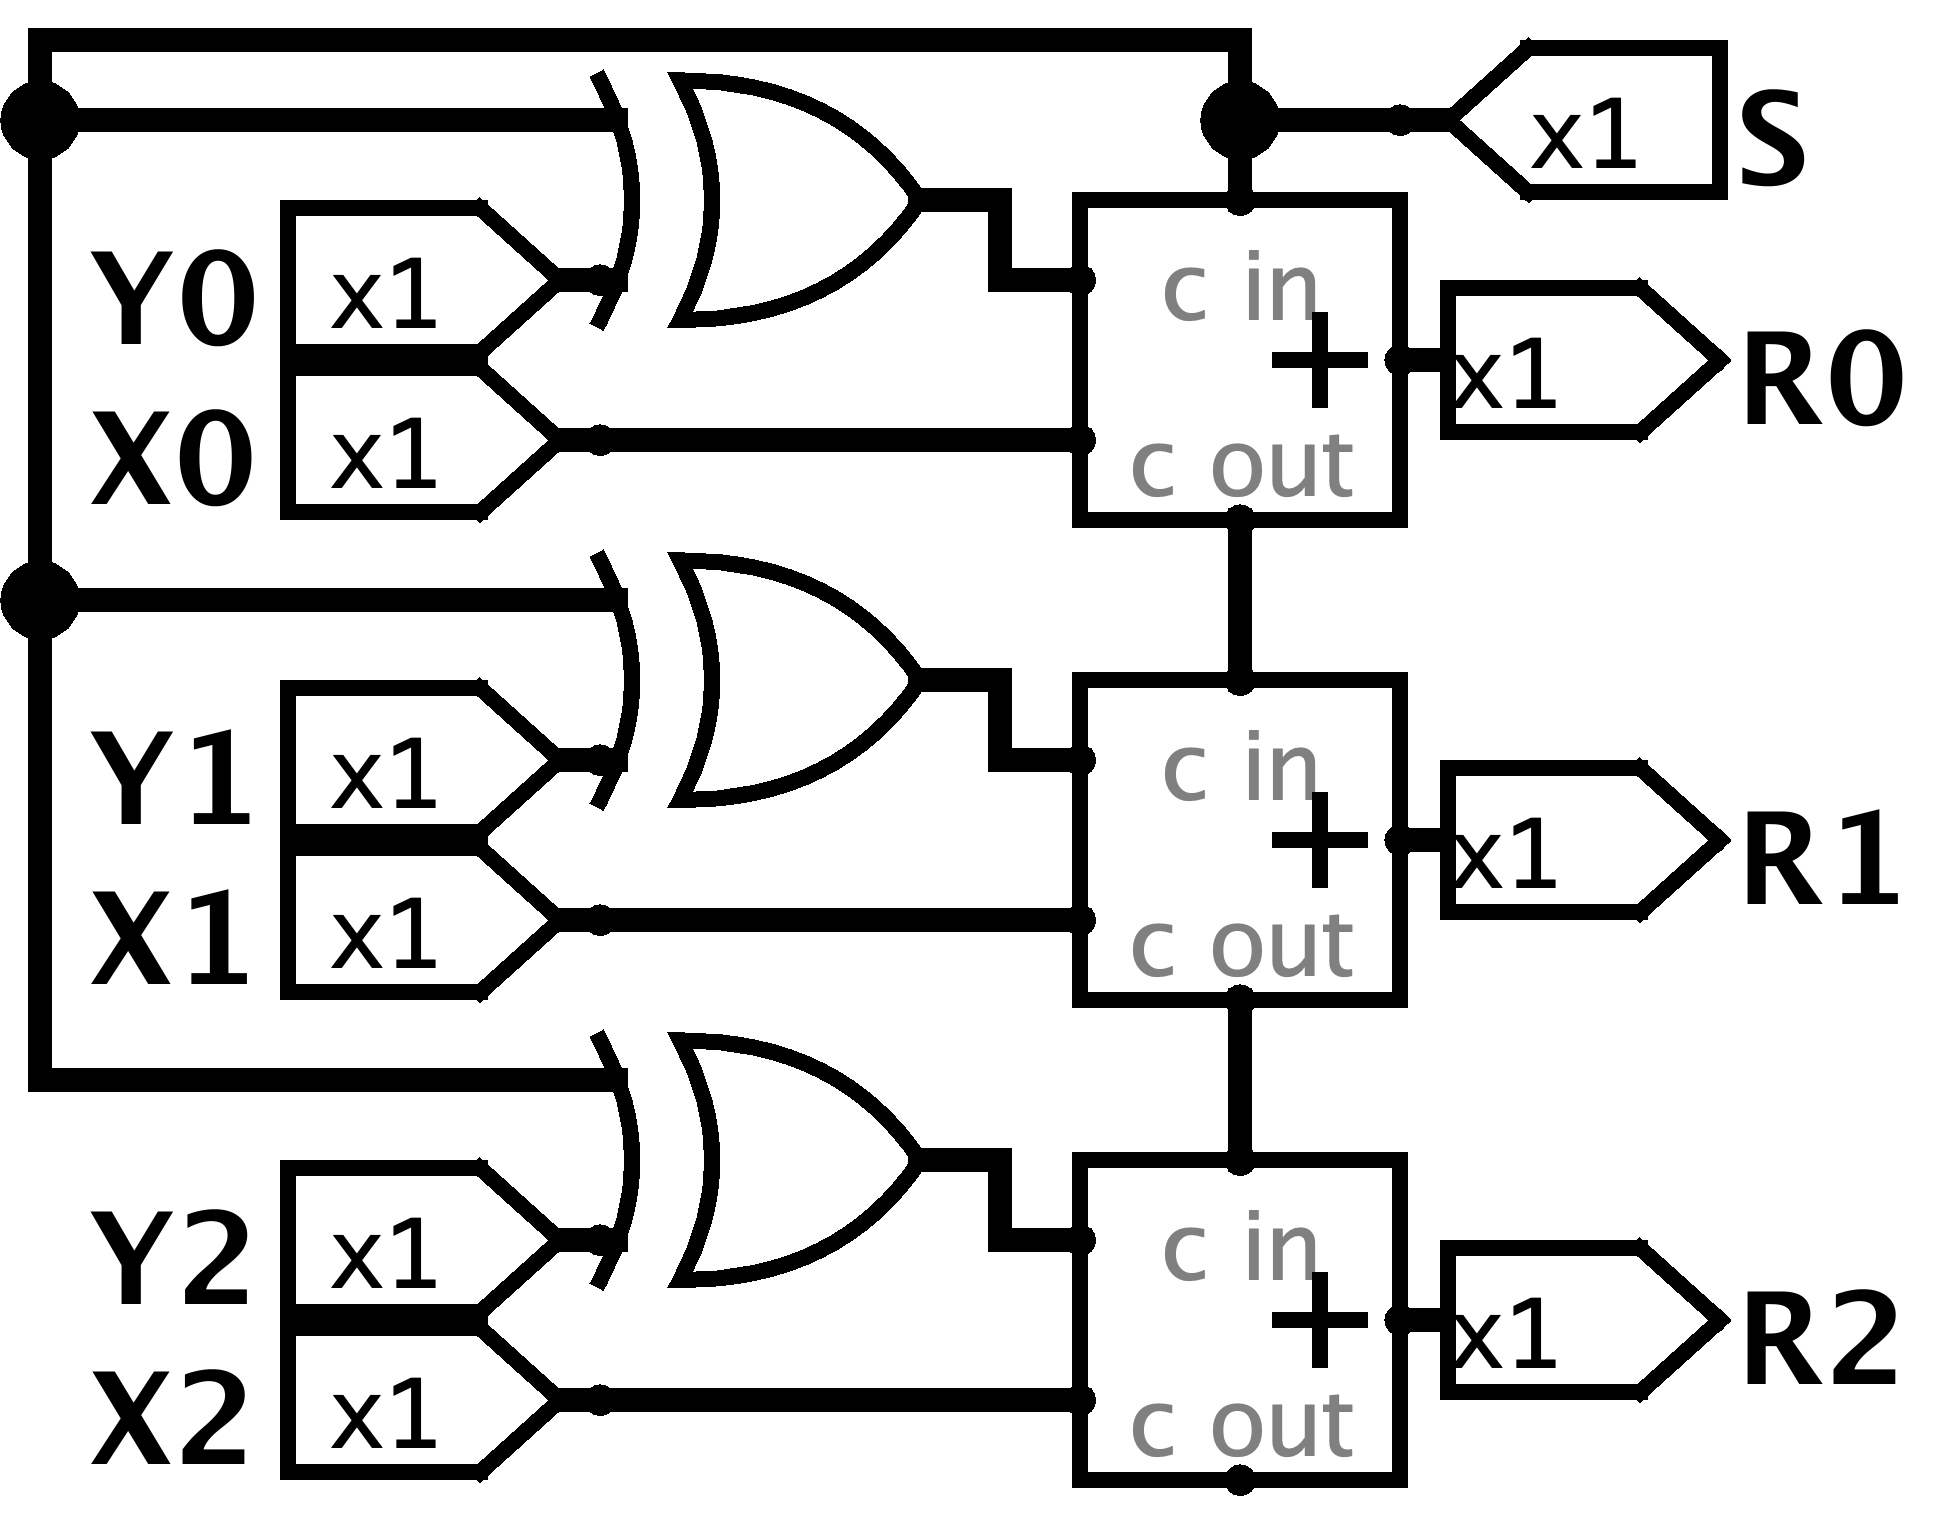
\includegraphics[width=0.75\linewidth]{resources/3Bit-Addierwerk.png}
\end{center}

\subsection*{4-Bit Paralleladdierwerk}

\begin{center}
    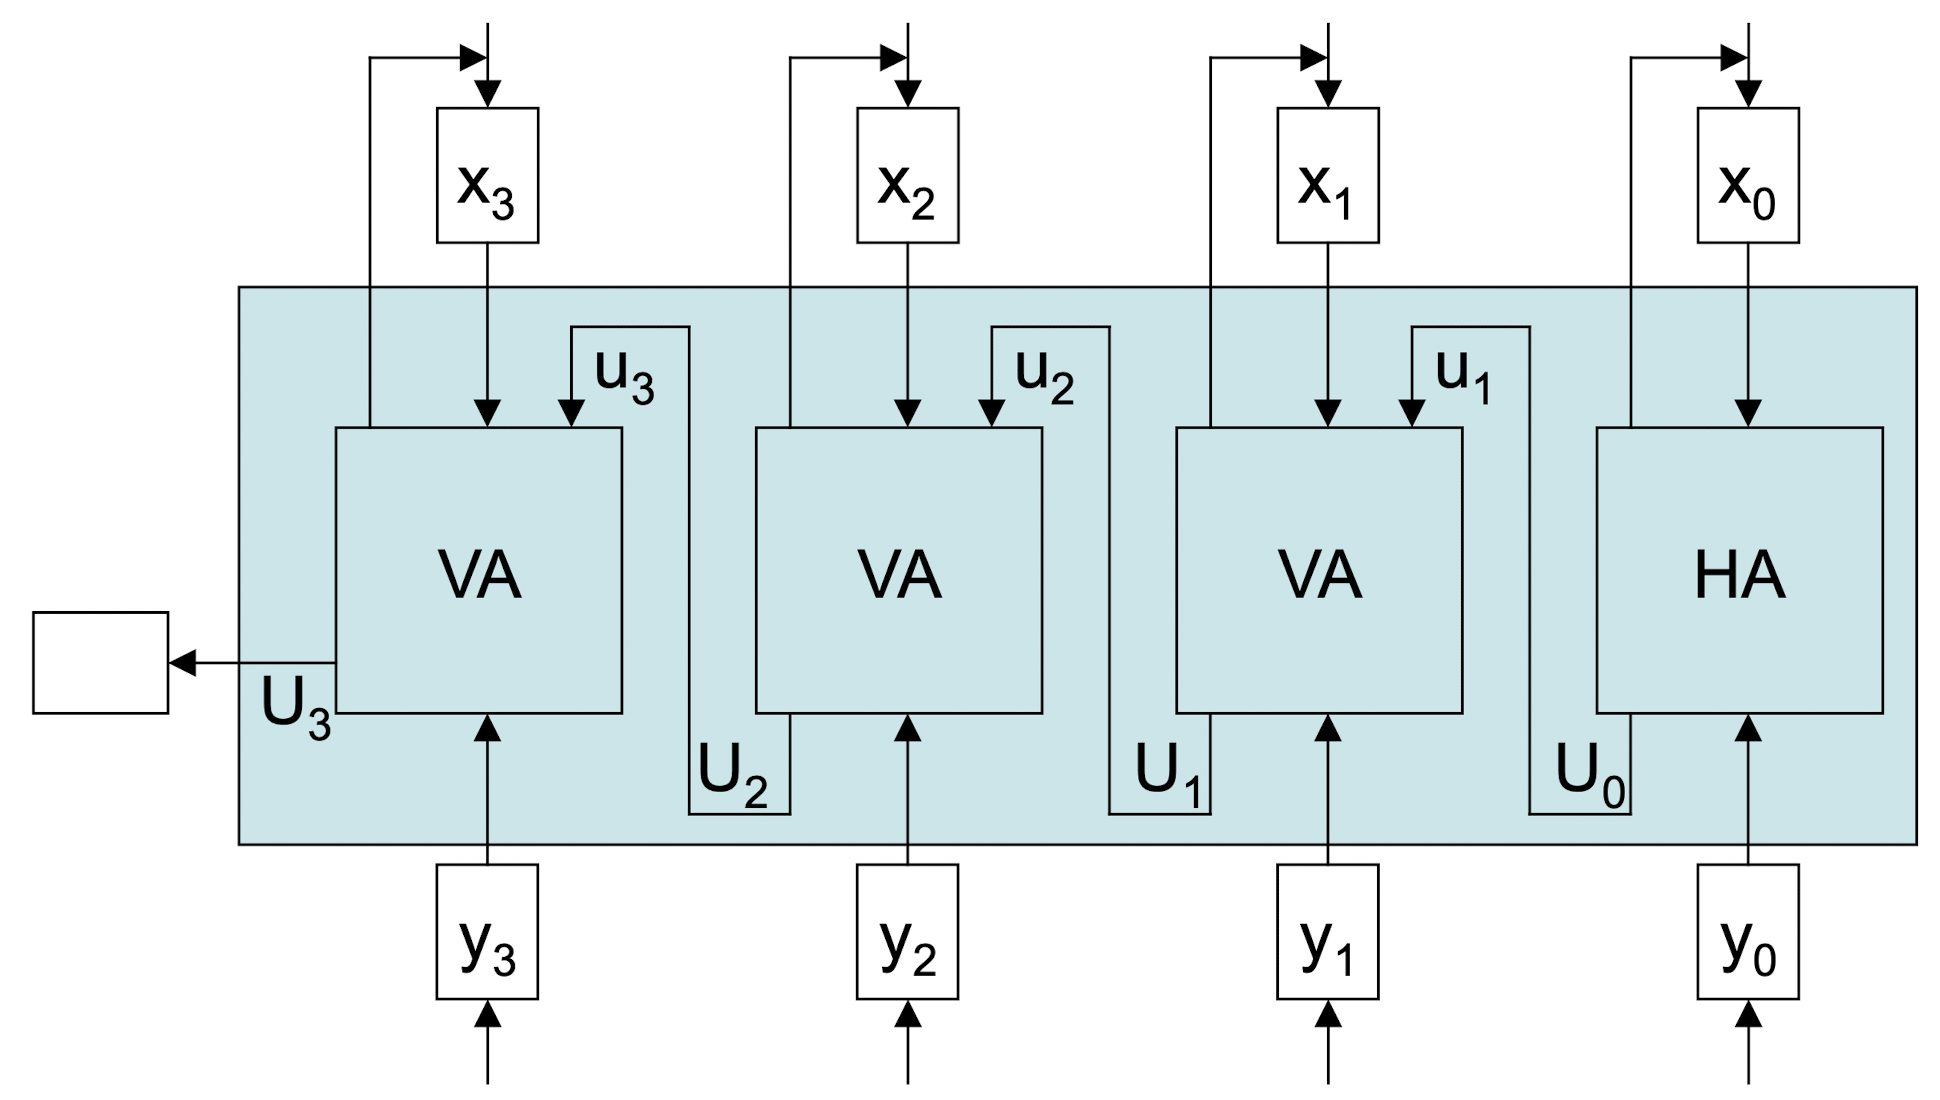
\includegraphics[width=1\linewidth]{resources/4Bit-Paralleladdierwerk.png}
\end{center}

\subsection*{4-Bit Serienaddierwerk}

\begin{center}
    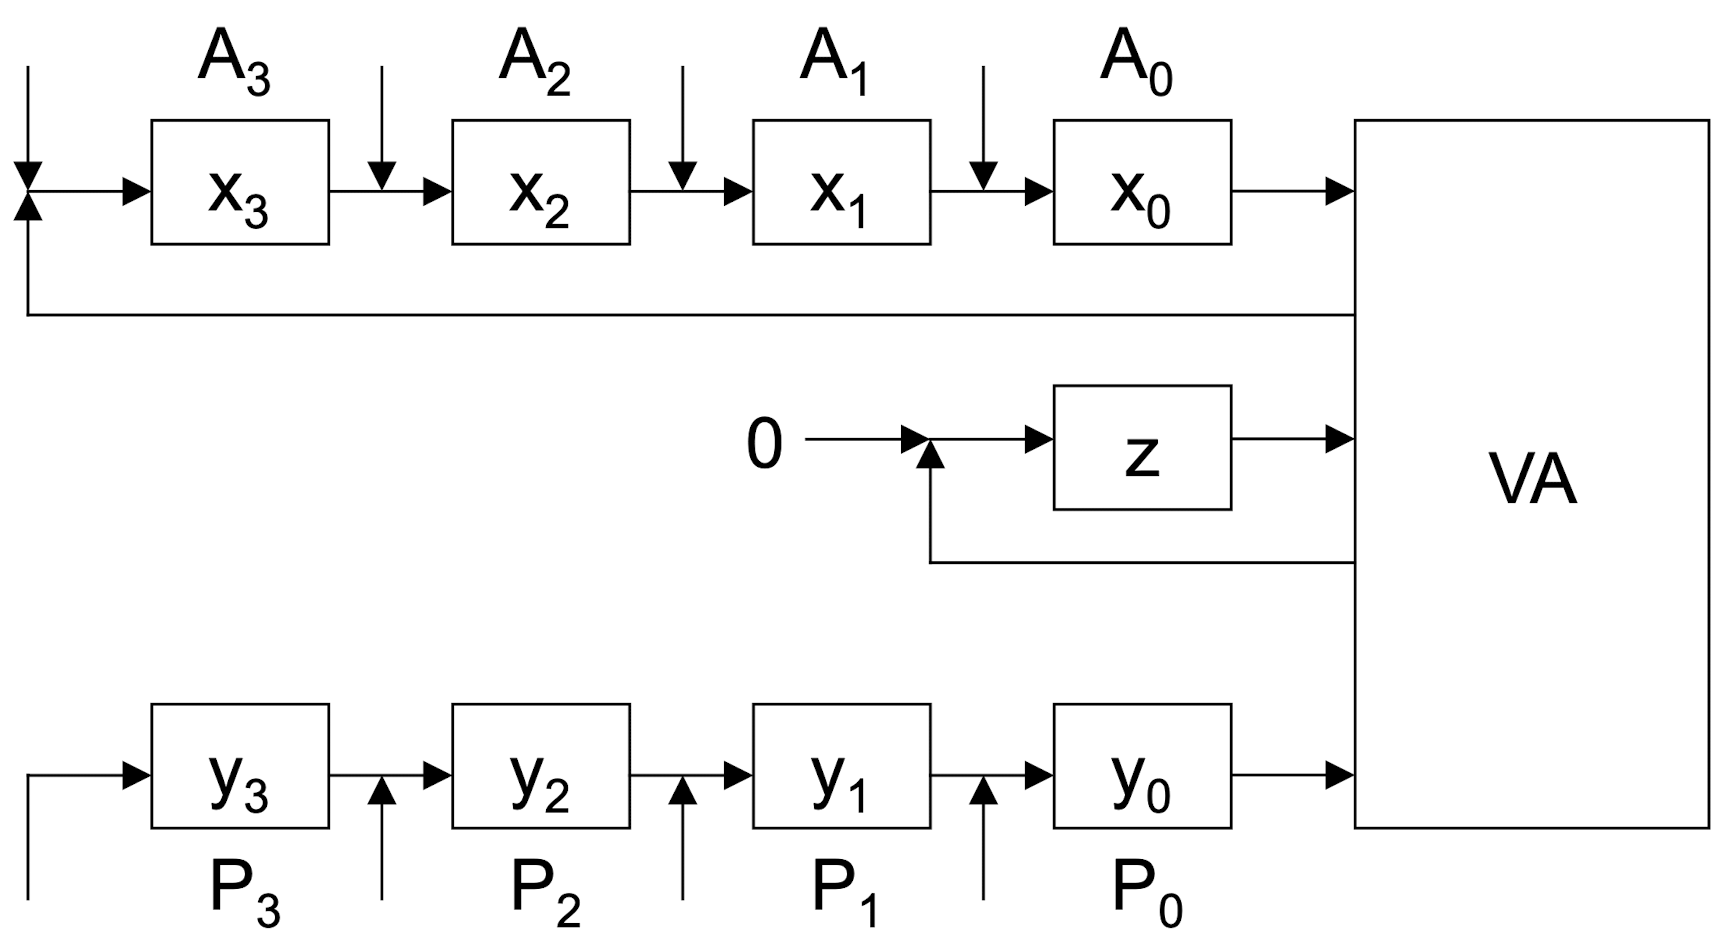
\includegraphics[width=1\linewidth]{resources/4Bit-Serienaddierwerk.png}
\end{center}

Ein $n$-Bit Serienaddierer benötigt $n + 1$ Schritte. $1$ Schritt für das Laden der Register und dann $n$ Addierschritte.

\subsection*{Linear rückgekoppeltes Schieberegister}

\begin{center}
    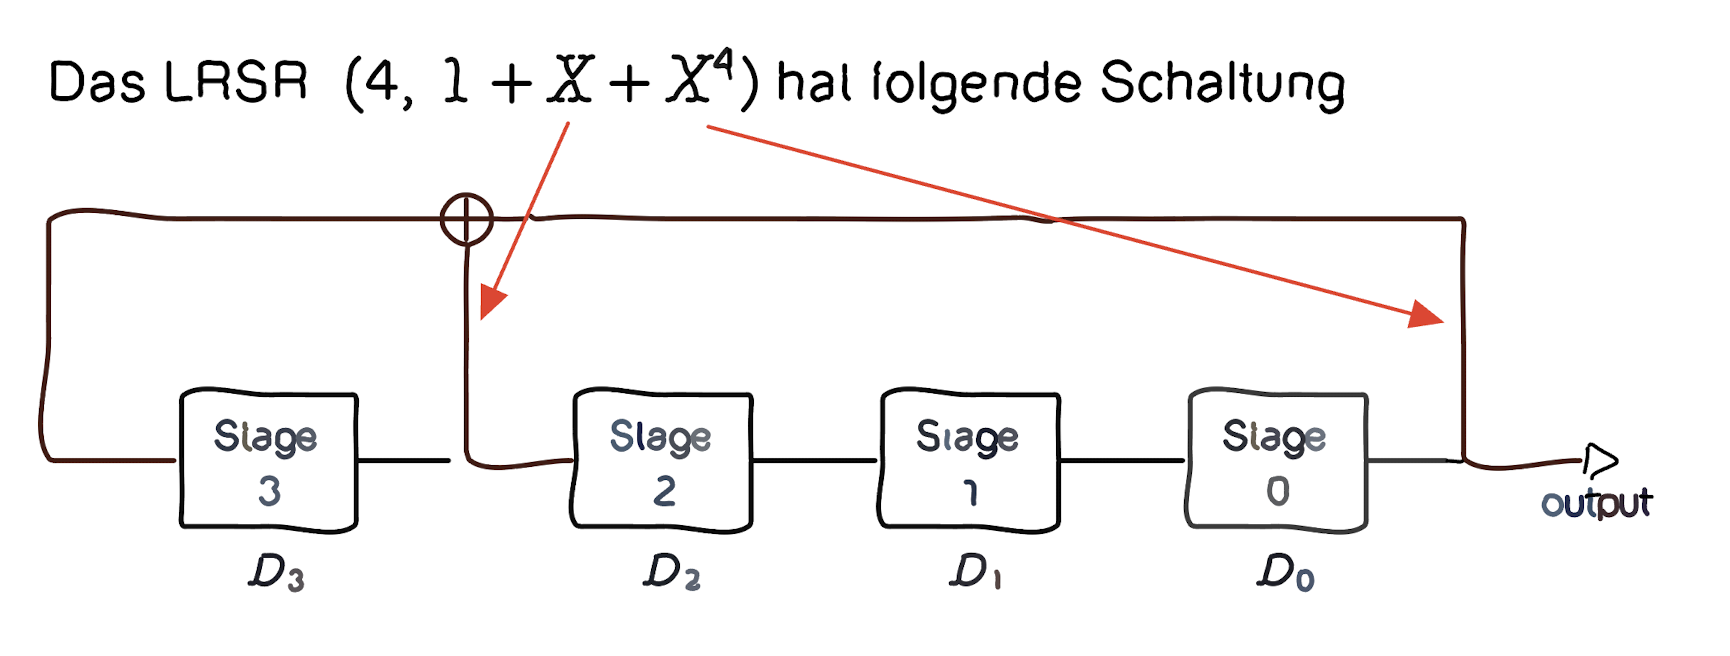
\includegraphics[width=1\linewidth]{resources/LRSR.png}
\end{center}

Keystream kann durch "rückwärts Einfädeln" überprüft werden.

\section{Gleitkommadarstellung}


\begin{equation*}
    z = \pm m \cdot b^{\pm e}
\end{equation*}

$m:$ Mantisse; $b:$ Basis; $e:$ Exponent

\subsection*{Nachkommastellen umrechnen}

\begin{align*}
    0.703125_{(10)} \times 2 &= \textbf{1}.40625_{(10)} \\
    0.40625_{(10)} \times 2 &= \textbf{0}.8125_{(10)} \\
    0.8125_{(10)} \times 2 &= \textbf{1}.625_{(10)} \\
    0.625_{(10)} \times 2 &= \textbf{1}.25_{(10)} \\
    0.25_{(10)} \times 2 &= \textbf{0}.5_{(10)} \\
    0.5_{(10)} \times 2 &= \textbf{1}.0_{(10)} \\
    0.703125_{(10)} &\rightarrow \textbf{0.1011010}_{(2)} \\
\end{align*}


\subsection*{Normalisierung}

\textit{Definition 1}

\begin{equation*}
    \frac{1}{b} \leq |m| < 1
\end{equation*}

\textit{Definition IEEE 754: }Eine Gleitkommazahl $\pm m \cdot 2^{\pm e}$ heisst normalisiert, falls $1 \leq m < 2$

Form: $(-1)^V \cdot 1.M \cdot 2^{E-\text{Basis}}$ wo $(\text{Basis} = 127; E = e + \text{Basis})$ 

1 Bit V + 8 Bit E + 23 Bit M
\begin{center}
    \begin{tabular}{|c|c|c|}
    \hline
    E & M & Bedeutung \\ \hline
    \(=255\) & \(\neq0\) & NAN / ungültig \\ \hline
    \(=255\) & \(=0\) & \(\pm\infty\) \\ \hline
    \(0 < E < 255\) & & \((-1)^V \cdot (1.M) \cdot 2^{E-127}\) \\ \hline
    \(=0\) & \(\neq0\) & \((-1)^V \cdot (0.M) \cdot 2^{-126}\) \\ \hline
    \(=0\) & \(=0\) & \(\pm0\) \\ \hline
    \end{tabular}
\end{center}

\section{ASCII}

\texttt{P000 0000}
\begin{itemize}
    \item $P = 0$: Anzahl von „1“-Bits ist gerade
    \item $P = 1$: Anzahl von „1“-Bits ist ungerade
\end{itemize}

\begin{center}
    \begin{tabular}{|c|l|}
    \hline
    Base 10 & Range \\ \hline
    0 - 31 & Control characters \\ \hline
    32 & Space \\ \hline
    33 - 47 & ! " \# \$ \% \& ' ( ) * + , - . / \\ \hline
    48 - 57 & 0 1 2 3 4 5 6 7 8 9 \\ \hline
    58 - 64 & : ; < = > ? @ \\ \hline
    65 - 90 & A - Z \\ \hline
    91 - 96 & [ \textbackslash ] \^ \_ ` \\ \hline
    97 - 122 & a - z \\ \hline
    123 - 126 & \{ | \} \textasciitilde \\ \hline
    127 & DEL \\ \hline
    \end{tabular}
\end{center}

\section{Multiplikation}

Carry-Save-Multilikation, gleich wie schriftliches Multiplizieren.
$$
\begin{array}{cccccccccc}
      &   &   &   & 1 & 0 & 1 & 1 &   & 11_{(10)} \\
      &   &   & \times & 1 & 1 & 0 & 1 &   & 13_{(10)} \\ \cline{1-8}
      &   &   &   & 1 & 0 & 1 & 1 &   &  \\
    + &   &   & 0 & 0 & 0 & 0 &   &   &  \\
    + &   & 1 & 0 & 1 & 1 &   &   &   &  \\
    + & 1 & 0 & 1 & 1 &   &   &   &   &  \\ \cline{1-8}
    1 & 1 & 1 & 1 &   &   &   &   &   &  \\ \cline{1-8}
    1 & 0 & 0 & 0 & 1 & 1 & 1 & 1 &   & 143_{(10)} \\ \cline{1-8} \cline{1-8}
\end{array}
$$

\begin{center}
    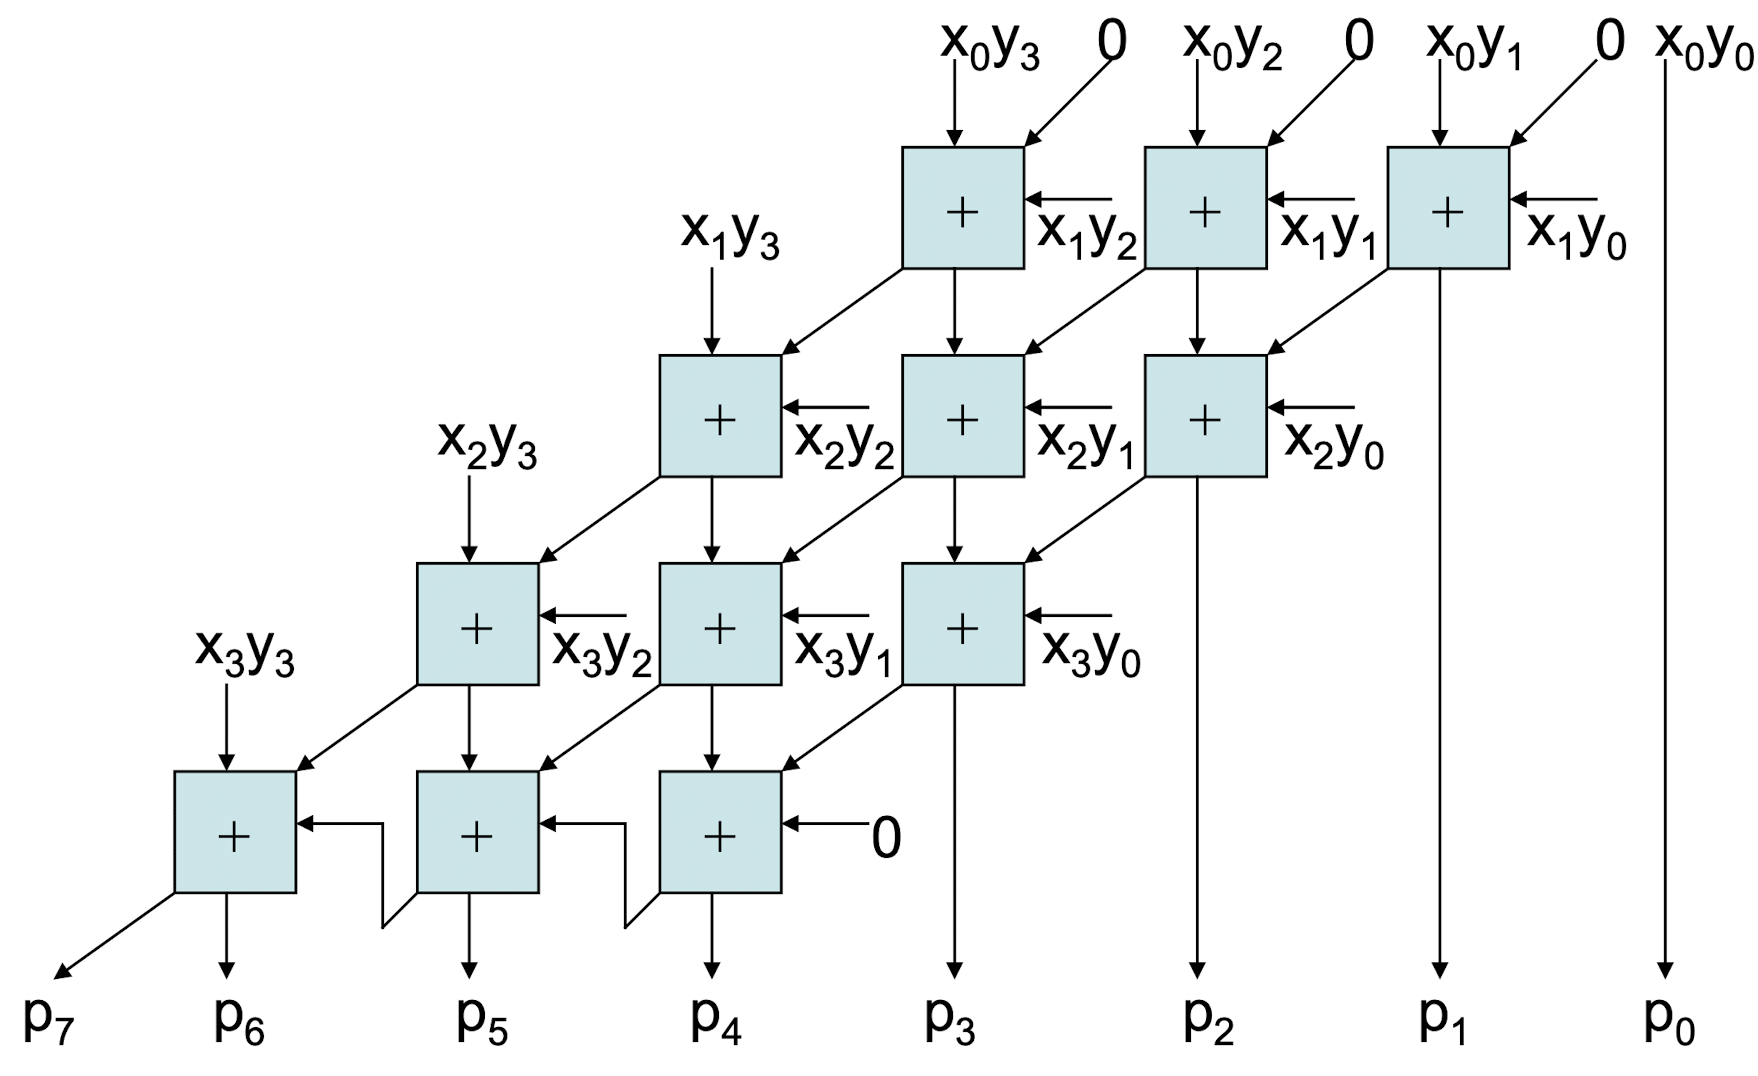
\includegraphics[width=1\linewidth]{resources/Multiplikation.png}
\end{center}

\section{Division}


\textbf{Wichtig:} Zuerst checken dass $2^4 d > z_{[5-8]}$ ansonsten Overflow

\textbf{Wichtig:} Zweierkomplement bilden für $-2^4 d$

\subsection*{Restoring Division}

\[
\setlength\arraycolsep{2pt} % Spaltenabstand anpassen
\begin{array}{lcccccccccccccc}
\hline
z                   & &   & & \textcolor{blue}{\textbf{0}} & \textcolor{blue}{\textbf{1}} & \textcolor{blue}{\textbf{1}} & \textcolor{blue}{\textbf{1}} & & 0 & 1 & 0 & 1 & = & 117_{(10)}  \\
2^4 d               & & 0 & & \textcolor{blue}{\textbf{1}} & \textcolor{blue}{\textbf{0}} & \textcolor{blue}{\textbf{1}} & \textcolor{blue}{\textbf{0}} & &   &   &   &   & = & 10_{(10)} \\
-2^4 d              & & 1 & & 0 & 1 & 1 & 0 & &   &   &   &   &   &   \\
\hline
s^{(0)}             & & 0 & & 0 & 1 & 1 & 1 & & 0 & 1 & 0 & 1 &   &   \\
2s^{(0)}            & & 1 & & 1 & 1 & 1 & 0 & & 1 & 0 & 1 &   &   &   \\
+(-2^4d)            & & 1 & & 0 & 1 & 1 & 0 & &   &   &   &   &   &   \\
\hline
s^{(1)}             & & 0 & & 0 & 1 & 0 & 0 & & 1 & 0 & 1 &   &   & q_3 = 1 \\
2s^{(1)}            & & 0 & & 1 & 0 & 0 & 1 & & 0 & 1 &   &   &   &   \\
+(-2^4d)            & & 1 & & 0 & 1 & 1 & 0 & &   &   &   &   &   &   \\
\hline
s^{(2)}             & & 1 & & 1 & 1 & 1 & 1 & & 0 & 1 &   &   &   & q_2 = 0 \\
s^{(2)}=2s^{(1)}    & & 0 & & 1 & 0 & 0 & 1 & & 0 & 1 &   &   &   &   \\
2s^{(2)}            & & 1 & & 0 & 0 & 1 & 0 & & 1 &   &   &   &   &   \\
+(-2^4d)            & & 1 & & 0 & 1 & 1 & 0 & &   &   &   &   &   &   \\
\hline
s^{(3)}             & & 0 & & 1 & 0 & 0 & 0 & & 1 &   &   &   &   & q_1 = 1 \\
2s^{(3)}            & & 1 & & 0 & 0 & 0 & 1 & &   &   &   &   &   &   \\
+(-2^4d)            & & 1 & & 0 & 1 & 1 & 0 & &   &   &   &   &   &   \\
\hline
s^{(4)}             & & 0 & & 0 & 1 & 1 & 1 & &   &   &   &   &   & q_0 = 1 \\
s                   & &   & &   &   &   &   & & 0 & 1 & 1 & 1 & = & 7_{(10)}  \\
q                   & &   & &   &   &   &   & & 1 & 0 & 1 & 1 & = & 11_{(10)} \\
\hline
\end{array}
\]


\subsection*{Non-restoring Division}

\[
\setlength\arraycolsep{2pt} % Spaltenabstand anpassen
\begin{array}{lcccccccccccccc}
\hline
z                   & &   & & \textcolor{blue}{\textbf{0}} & \textcolor{blue}{\textbf{1}} & \textcolor{blue}{\textbf{1}} & \textcolor{blue}{\textbf{0}} & & 1 & 0 & 0 & 1 & = & 100_{(10)} \\
2^4 d               & & 0 & & \textcolor{blue}{\textbf{1}} & \textcolor{blue}{\textbf{0}} & \textcolor{blue}{\textbf{0}} & \textcolor{blue}{\textbf{1}} & &   &   &   &   & = & 9_{(10)} \\
-2^4 d              & & 1 & & 0 & 1 & 1 & 1 & &   &   &   &   &   &   \\
\hline
s^{(0)}             & & 0 & & 0 & 1 & 1 & 0 & & 0 & 1 & 0 & 0 &   &   \\
2s^{(0)}            & & 0 & & 1 & 1 & 0 & 0 & & 1 & 0 & 0 &   &   &   \\
+(-2^4d)            & & 1 & & 0 & 1 & 1 & 1 & &   &   &   &   &   &   \\
\hline
s^{(1)}             & & 0 & & 0 & 0 & 1 & 1 & & 0 & 0 &   &   &   & q_3 = 1 \\
2s^{(1)}            & & 0 & & 0 & 1 & 1 & 1 & & 0 & 0 &   &   &   &   \\
+(-2^4d)            & & 1 & & 0 & 1 & 1 & 1 & &   &   &   &   &   &   \\
\hline
s^{(2)}             & & 1 & & 1 & 1 & 1 & 0 & & 0 & 0 &   &   &   & q_2 = 0 \\
2s^{(2)}            & & 1 & & 1 & 1 & 0 & 0 & & 0 &   &   &   &   &   \\
+2^4d               & & 0 & & 1 & 0 & 0 & 1 & &   &   &   &   &   &   \\
\hline
s^{(3)}             & & 0 & & 0 & 1 & 0 & 1 & & 0 &   &   &   &   & q_1 = 1 \\
2s^{(3)}            & & 0 & & 1 & 0 & 1 & 0 & &   &   &   &   &   &   \\
+(-2^4d)            & & 1 & & 0 & 1 & 1 & 1 & &   &   &   &   &   &   \\
\hline
s^{(4)}             & & 0 & & 0 & 0 & 0 & 1 & &   &   &   &   &   & q_0 = 1 \\
s                   & &   & &   &   &   &   & & 0 & 0 & 0 & 1 & = & 1_{(10)}   \\
q                   & &   & &   &   &   &   & & 1 & 0 & 1 & 1 & = & 11_{(10)}  \\
\hline
\end{array}
\]


\section{Model checking}

\subsection*{Erreichbarkeitsanalyse}

Gegeben seien die Inputmenge \( I = \{0, 1\} \), die Zustandsmenge \( Q = \{0, 1\}^4 \) und die Übergangsfunktion \( d : I \times Q \rightarrow Q \) mit


\[
d(0; q_1, q_2, q_3, q_4) = 
\begin{cases}
    (q_1 q_2 q_3 q_4)_2 + (100)_2 & \text{if } < 16 \\
    (0, 0, 0, 0) & \text{else}
\end{cases}
\]

\[
d(1; q_1, q_2, q_3, q_4) = 
\begin{cases}
    (q_1 q_2 q_3 q_4)_2 + (101)_2 & \text{if } < 16 \\
    (0, 0, 0, 0) & \text{else}
\end{cases}
\]

\begin{align*}
    \text{Start:} &= (0,1,0,0) \\
    S_0 = \{&(0,1,0,0)\} \\
    \\
    d(0;0,1,0,0) &= (1,0,0,0) \\
    d(1;0,1,0,0) &= (1,0,0,1) \\
    S_1 = S_0 \cup \{&(1,0,0,0),(1,0,0,1)\} \\
    \\
    d(0;1,0,0,0) &= (1,1,0,0) \\
    d(0;1,0,0,1) &= (1,1,0,1) \\
    d(1;1,0,0,0) &= (1,1,0,1) \\
    d(1;1,0,0,1) &= (1,1,1,0) \\
    S_2 = S_1 \cup \{(1,1,0,0),&(1,1,0,1),(1,1,1,0)\} \\
    &\vdots \\
    S_{n + 1} = S_{n} \rightarrow &\textbf{terminieren} \\
    \\
     S = \{(0,0,0,0),(0,1,0,0)&,(1,0,1,0),(1,0,0,0), \\
    (1,0,0,1),(1,0,1,0)&,(1,1,0,0),(1,1,0,1), \\
    (1,1,1,0),(1,1,1,1)&\} \\
    (1,0,1,1) \notin S&
\end{align*}

\section{CTL}

\begin{itemize}
    \item $E X \phi$: es gibt einen Pfad, auf dem als nächstes $\phi$ wahr ist
    \item $A X \phi$: auf jedem Pfad ist als nächstes $\phi$ wahr
    \item $E F \phi$: es gibt einen Pfad auf dem irgendwann $\phi$ wahr ist
    \item $A F \phi$: auf allen Pfaden ist $\phi$ irgendwann wahr
    \item $E G \phi$: es gibt einen Pfad, auf dem $\phi$ immer wahr ist
    \item $A G \phi$: auf allen Pfaden ist $\phi$ immer wahr
    \item $\phi E U \psi$: es gibt einen Pfad, auf dem $\phi$ wahr bleibt, bis $\psi$ wahr wird
    \item $\phi A U \psi$: auf allen Pfaden bleibt $\phi$ wahr, bis $\psi$ wahr wird
\end{itemize}

\begin{center}
    \begin{tabular}{c|l}
    \textbf{Symbol} & \textbf{Bedeutung} \\
    \hline
    \( \top \) & Wahr (True) \\
    \( \bot \) & Falsch (False) \\
    \( \neg \) & Negation (Not) \\
    \( \wedge \) & Konjunktion (And) \\
    \( \vee \) & Disjunktion (Or) \\
    \( \rightarrow \) & Implikation \\
    \( \leftrightarrow \) & Äquivalenz (If and only if) \\
    \( p \) & Eine atomare Proposition \\
    \( L(v) \) & Labeling-Funktion \\
    \( I \) & Anfangszustände (Initial states) \\
    \( \pi \) & Ein Pfad \\
    \( \pi_i \) & Die \(i\)-te Stelle in einem Pfad \\
    \( \mathcal{P}(\mathit{Prop}) \) & Potenzmenge d. atom. Propositionen \\
    \( V \) & Knoten (States) \\
    \( E \) & Kanten (Transitions) \\
    \end{tabular}
\end{center}

\begin{itemize}
    \item Auf jedem Pfad ist es immer möglich, dass $p$ irgendwann wahr wird:
    \begin{itemize}
        \item[$\rightarrow$] $\text{AG EF } p$
    \end{itemize}
    \item $p$ ist möglich:
    \begin{itemize}
        \item[$\rightarrow$] $\text{EF } p$
    \end{itemize}
    \item $p$ und $q$ sind nie gleichzeitig wahr:
    \begin{itemize}
        \item[$\rightarrow$] $\text{AG}\neg(p \wedge q)$ oder $\neg\text{EF}(p \wedge q)$
    \end{itemize}
    \item Auf jedem Pfad ist $p$ unendlich oft wahr:
    \begin{itemize}
        \item[$\rightarrow$] $\text{AG AF } p$
    \end{itemize}
    \item $p$ und immer falls $p$ dann direkt danach $p$, impliziert $p$ gilt immer (Induktion):
    \begin{itemize}
        \item[$\rightarrow$] $p \wedge \text{AG}(p \rightarrow \text{AX}p) \rightarrow \text{AG}p$
    \end{itemize}
    \item Auf jedem Pfad sind $p$ und $q$ abwechselnd wahr, wobei jeweils nur eine der beiden Propositionen wahr ist:
    \begin{itemize}
        \item[$\rightarrow$] $(p \wedge \neg q) \vee (\neg p \wedge q) \wedge \text{AG}((p \rightarrow \text{AX}(\neg p \wedge q)) \wedge (q \rightarrow \text{AX}(p \wedge \neg q)))$
    \end{itemize}
    \item Sei $p =$ 'Es regnet'. Es regnet und es wird weiterregnen, bis es aufgehört hat, zu regnen:
    \begin{itemize}
        \item[$\rightarrow$] $p \wedge (p \text{ AU } \neg p)$
    \end{itemize}
\end{itemize}

\subsection*{Algorithmus}

\textbf{Reduktionen}

\begin{itemize}
    \item $AX \varphi \Leftrightarrow \neg EX \neg \varphi$
        \begin{itemize}
            \item \tiny{Wenn $AX \varphi$ wahr ist, dann gibt es keinen Pfad, auf dem als nächstes $\neg \varphi$ wahr ist.}
        \end{itemize}
    \item $AG \varphi \Leftrightarrow \neg EF \neg \varphi$
        \begin{itemize}
            \item \tiny{Wenn $AG \varphi$ wahr ist, dann gibt es keinen Pfad, auf dem irgendwann $\neg \varphi$ wahr ist.}
        \end{itemize}
    \item $EF \varphi \Leftrightarrow T EU \varphi$
        \begin{itemize}
            \item \tiny{Wenn $EF \varphi$ wahr ist, dann ist von einem wahren Zustand aus $\varphi$ irgendwann erreichbar.}
        \end{itemize}
    \item $EG \varphi \Leftrightarrow \neg AF \neg \varphi$
        \begin{itemize}
            \item \tiny{Wenn $EG \varphi$ wahr ist, dann ist $\varphi$ immer wahr auf einem Pfad, auf dem $\neg \varphi$ nicht irgendwann wahr wird.}
        \end{itemize}
    \item $\varphi AU \psi \Leftrightarrow \neg ((\neg \psi) EU (\neg (\varphi \lor \psi))) \land AF \psi$
        \begin{itemize}
            \item \tiny{Wenn $\varphi AU \psi$ wahr ist, dann gibt es keinen Pfad, auf dem $\neg \psi$ bleibt, bis $\neg (\varphi \lor \psi)$ wahr wird, und irgendwann wird $\psi$ wahr.}
        \end{itemize}
\end{itemize}

Hierbei ist $T$ definiert als $T := p_0 \lor \neg p_0$, was immer wahr ist.

Der Algorithmus behandelt:
\[ \neg, \wedge, \text{EX}, \text{EU}, \text{AF} \]
Es gilt:
\begin{align*}
\text{AX}\Phi &\equiv \neg \text{EX}\neg \Phi \\
\text{AG}\Phi &\equiv \neg \text{EF}\neg \Phi \\
\text{EF}\Phi &\equiv \top \text{EU}\Phi \\
\text{EG}\Phi &\equiv \neg \text{AF}\neg \Phi \\
\Phi \text{AU}\Psi &\equiv \neg(\neg \Psi \text{EU} \neg(\Phi \vee \Psi)) \wedge \text{AF}\Psi \\
\Phi \rightarrow \Psi &\equiv \neg \Phi \vee \Psi \\
\Phi \vee \Psi &\equiv \neg(\neg \Phi \wedge \neg \Psi)
\end{align*}


\section{ALU}

Most-significant-Bit
\begin{center}
    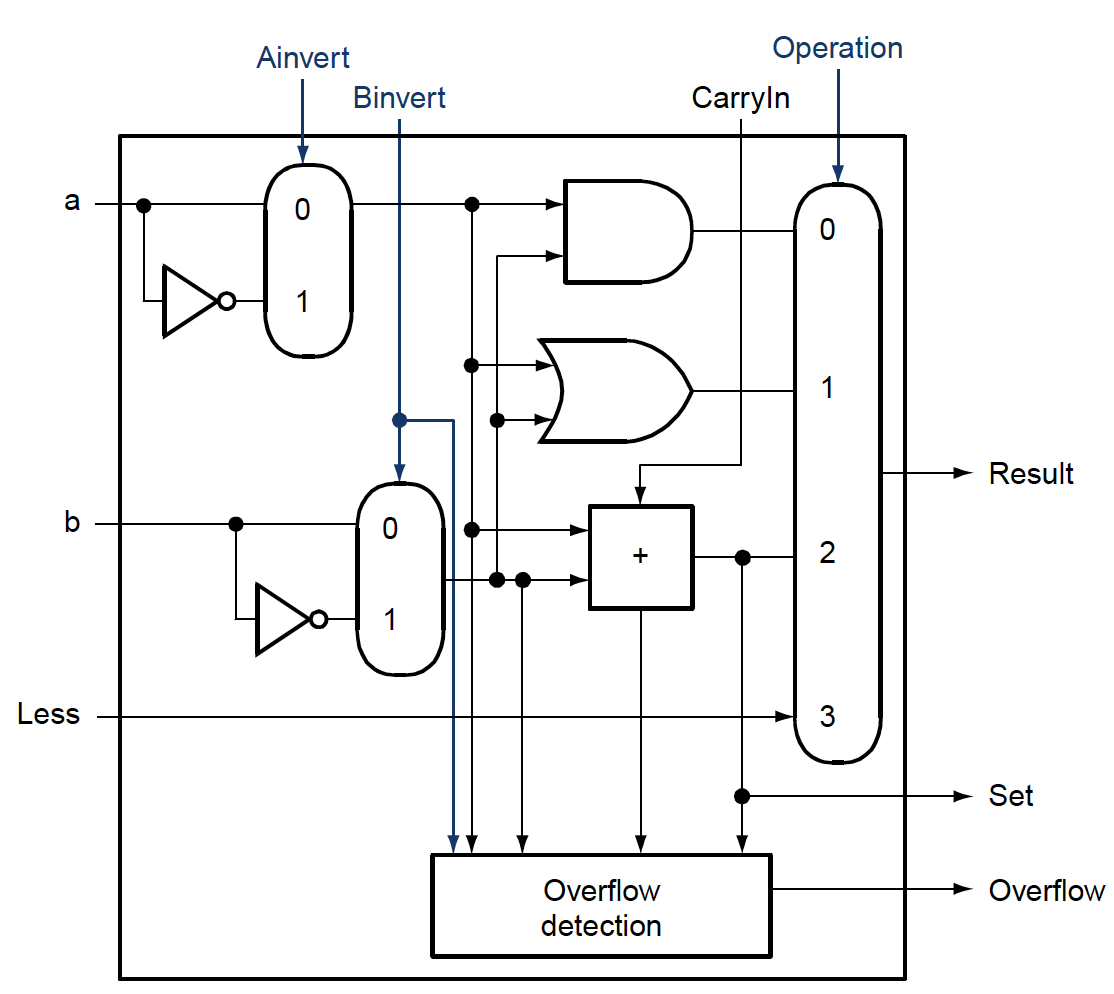
\includegraphics[width=1\linewidth]{resources/MostSignificantBit.png}
\end{center}

Every other Bit
\begin{center}
    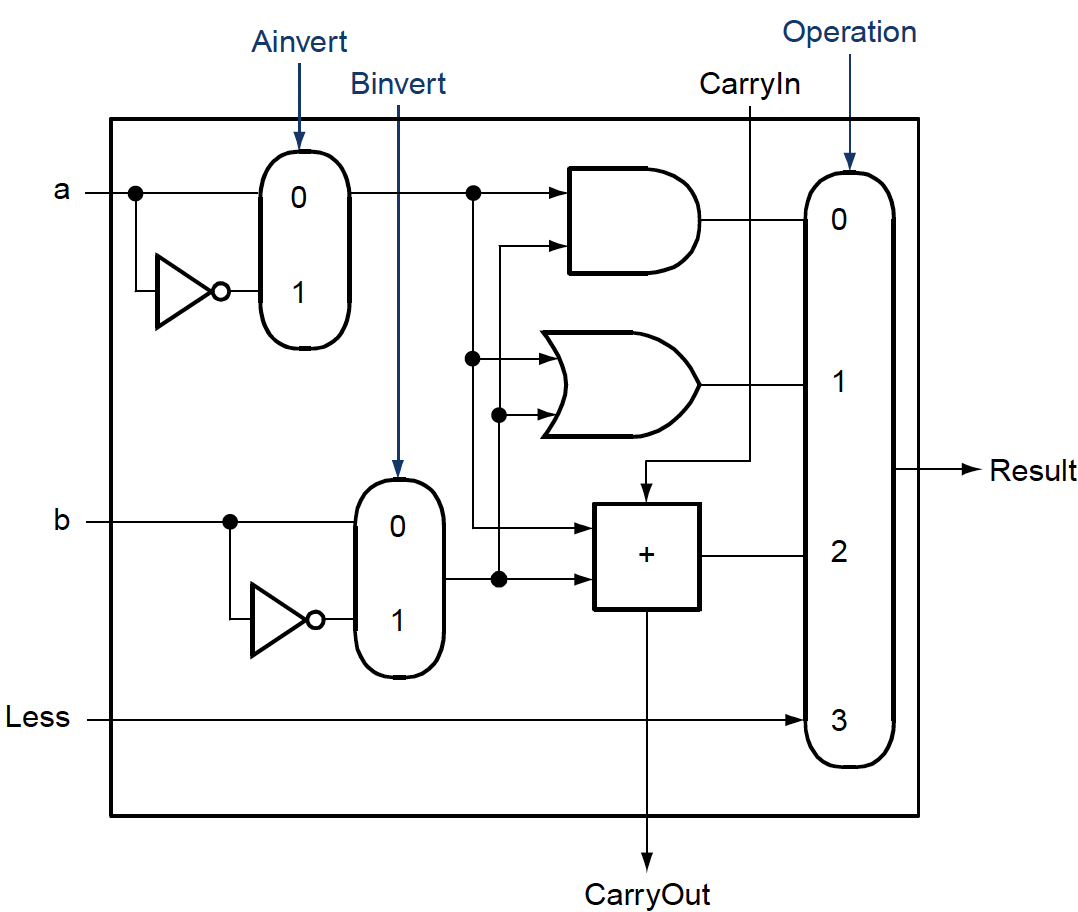
\includegraphics[width=1\linewidth]{resources/ALU_EveryOtherBit.png}
\end{center}

Komplettes ALU (bemerke $\neg B$ als $c_{in}$ im least-significant-bit für 2-er Komplement)
\begin{center}    
    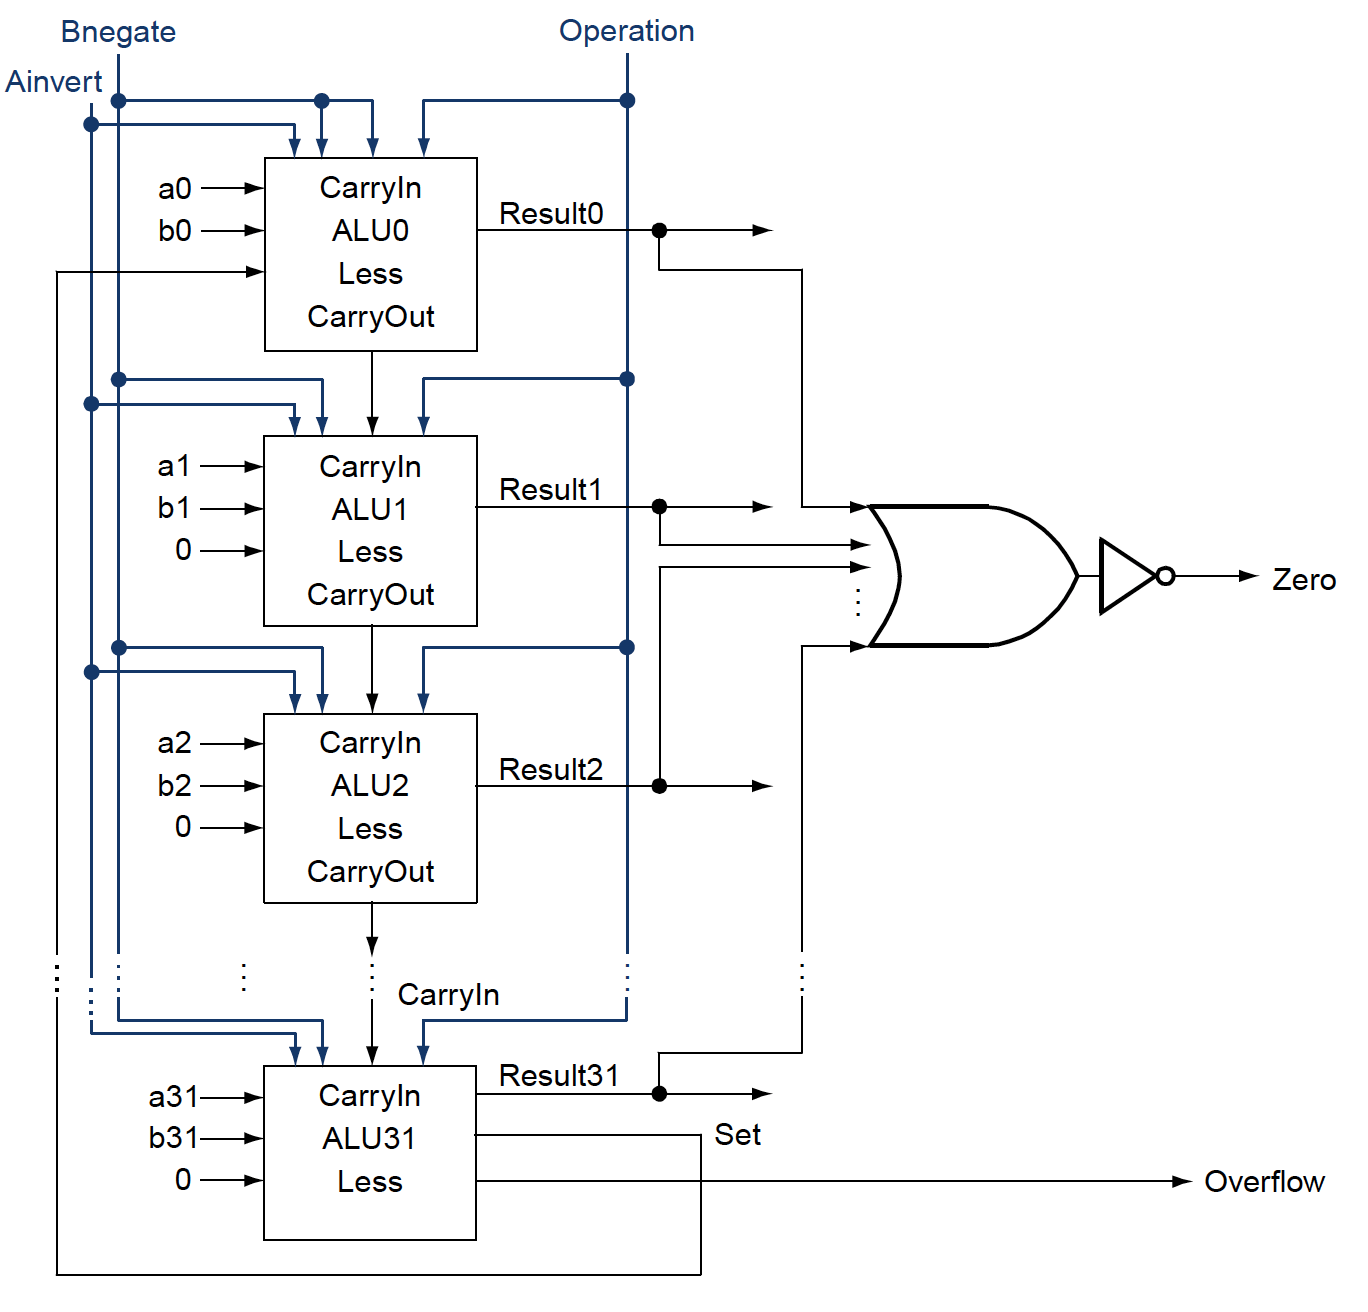
\includegraphics[width=1\linewidth]{resources/ALU_Complete.png}
\end{center}

$$
slt(a,b) :=
\begin{cases}
    0 \quad \text{sonst} \\
    1 \quad \text{wenn } a < b \\
\end{cases}
$$


\end{multicols*}
\end{document}
